\documentclass{article}

% if you need to pass options to natbib, use, e.g.:
%     \PassOptionsToPackage{numbers, compress}{natbib}
% before loading neurips_2025

% The authors should use one of these tracks.
% Before accepting by the NeurIPS conference, select one of the options below.
% 0. "default" for submission
% \usepackage{neurips_2025}
% the "default" option is equal to the "main" option, which is used for the Main Track with double-blind reviewing.
% 1. "main" option is used for the Main Track
%  \usepackage[main]{neurips_2025}
% 2. "position" option is used for the Position Paper Track
%  \usepackage[position]{neurips_2025}
% 3. "dandb" option is used for the Datasets & Benchmarks Track
 % \usepackage[dandb]{neurips_2025}
% 4. "creativeai" option is used for the Creative AI Track
%  \usepackage[creativeai]{neurips_2025}
% 5. "sglblindworkshop" option is used for the Workshop with single-blind reviewing
 % \usepackage[sglblindworkshop]{neurips_2025}
% 6. "dblblindworkshop" option is used for the Workshop with double-blind reviewing
%  \usepackage[dblblindworkshop]{neurips_2025}

% After being accepted, the authors should add "final" behind the track to compile a camera-ready version.
% 1. Main Track
\usepackage[main, final]{neurips_2025}
% 2. Position Paper Track
%  \usepackage[position, final]{neurips_2025}
% 3. Datasets & Benchmarks Track
 % \usepackage[dandb, final]{neurips_2025}
% 4. Creative AI Track
%  \usepackage[creativeai, final]{neurips_2025}
% 5. Workshop with single-blind reviewing
%  \usepackage[sglblindworkshop, final]{neurips_2025}
% 6. Workshop with double-blind reviewing
%  \usepackage[dblblindworkshop, final]{neurips_2025}
% Note. For the workshop paper template, both \title{} and \workshoptitle{} are required, with the former indicating the paper title shown in the title and the latter indicating the workshop title displayed in the footnote.
% For workshops (5., 6.), the authors should add the name of the workshop, "\workshoptitle" command is used to set the workshop title.
% \workshoptitle{WORKSHOP TITLE}

% "preprint" option is used for arXiv or other preprint submissions
 % \usepackage[preprint]{neurips_2025}

% to avoid loading the natbib package, add option nonatbib:
%    \usepackage[nonatbib]{neurips_2025}

\usepackage[utf8]{inputenc} % allow utf-8 input
\usepackage[T1]{fontenc}    % use 8-bit T1 fonts
\usepackage{hyperref}       % hyperlinks
\usepackage{url}            % simple URL typesetting
\usepackage{booktabs}       % professional-quality tables
\usepackage{amsfonts}       % blackboard math symbols
\usepackage{nicefrac}       % compact symbols for 1/2, etc.
\usepackage{microtype}      % microtypography
\usepackage{xcolor}         % colors
\usepackage{mathtools}
\usepackage{amsmath,amssymb,amsthm}
\usepackage{cleveref}
\usepackage{algorithm}
\usepackage{algpseudocode}
\usepackage{graphicx}
\usepackage{subcaption}
\usepackage{tikz}
\usepackage{xcolor}
\usepackage{subcaption}
\captionsetup[subfigure]{skip=-7pt}
\usetikzlibrary{calc}

\newtheorem{theorem}{Theorem}
\newtheorem{lemma}{Lemma} 
\newtheorem{proposition}{Proposition} 
\newtheorem{corollary}{Corollary}
\newtheorem{definition}{Definition} 
\newtheorem{example}{Example} 
\newtheorem{assumption}{Assumption}
\newtheorem{claim}{Claim}
\newtheorem{remark}{Remark}
\newtheorem{note}{Note} 
\newtheorem{question}{Question}

\crefname{theorem}{Theorem}{Theorems}
\Crefname{theorem}{Theorem}{Theorems}

\crefname{lemma}{Lemma}{Lemmas}
\Crefname{lemma}{Lemma}{Lemmas}

\crefname{proposition}{Proposition}{Propositions}
\Crefname{proposition}{Proposition}{Propositions}

\crefname{corollary}{Corollary}{Corollaries}
\Crefname{corollary}{Corollary}{Corollaries}

\crefname{definition}{Definition}{Definitions}
\Crefname{definition}{Definition}{Definitions}

\crefname{example}{Example}{Examples}
\Crefname{example}{Example}{Examples}

\crefname{assumption}{Assumption}{Assumptions}
\Crefname{assumption}{Assumption}{Assumptions}

\crefname{claim}{Claim}{Claims}
\Crefname{claim}{Claim}{Claims}

\crefname{remark}{Remark}{Remarks}
\Crefname{remark}{Remark}{Remarks}

\crefname{note}{Note}{Notes}
\Crefname{note}{Note}{Notes}

\crefname{question}{Question}{Questions}
\Crefname{question}{Question}{Questions}

\DeclareMathOperator*{\argmin}{arg\,min}
\DeclareMathOperator*{\argmax}{arg\,max}

% Note. For the workshop paper template, both \title{} and \workshoptitle{} are required, with the former indicating the paper title shown in the title and the latter indicating the workshop title displayed in the footnote. 
\title{Learning Geometry Preserving Optimal Transport Plan via Convex Relaxation}


% The \author macro works with any number of authors. There are two commands
% used to separate the names and addresses of multiple authors: \And and \AND.
%
% Using \And between authors leaves it to LaTeX to determine where to break the
% lines. Using \AND forces a line break at that point. So, if LaTeX puts 3 of 4
% authors names on the first line, and the last on the second line, try using
% \AND instead of \And before the third author name.


\author{%
  Junhyoung Chung\thanks{\href{https://junhyoung-chung.github.io/}{https://junhyoung-chung.github.io/}} \\
  Department of Statistics\\
  Seoul National University\\
  Seoul 08826, Republic of Korea \\
  \texttt{junhyoung0534@gmail.com} \\
  % examples of more authors
  % \And
  % Coauthor \\
  % Affiliation \\
  % Address \\
  % \texttt{email} \\
  % \AND
  % Coauthor \\
  % Affiliation \\
  % Address \\
  % \texttt{email} \\
  % \And
  % Coauthor \\
  % Affiliation \\
  % Address \\
  % \texttt{email} \\
  % \And
  % Coauthor \\
  % Affiliation \\
  % Address \\
  % \texttt{email} \\
}


\begin{document}


\maketitle


\begin{abstract}
  The abstract paragraph should be indented \nicefrac{1}{2}~inch (3~picas) on
  both the left- and right-hand margins. Use 10~point type, with a vertical
  spacing (leading) of 11~points.  The word \textbf{Abstract} must be centered,
  bold, and in point size 12. Two line spaces precede the abstract. The abstract
  must be limited to one paragraph.
\end{abstract}


\section{Introduction}

Optimal transport (OT) is a foundational tool for comparing probability measures by accounting for the cost of moving mass across spaces~\citep{villani2008optimal}. Beyond classical settings where distributions live in Euclidean domains, modern applications in statistics, machine learning, and computer vision routinely involve signals supported on non-Euclidean or structured spaces (e.g., meshes, graphs, manifolds) together with auxiliary features (descriptors). In such problems, meaningful alignment must jointly respect (i) feature correspondence and (ii) the geometry of the underlying domain.

A popular way to incorporate geometry is the Gromov--Wasserstein (GW) framework, which matches distributions by comparing within-domain pairwise distances. More recently, the fused GW (FGW) discrepancy~\citep{vayer2020fused} blends feature matching with GW, offering a flexible interpolation. However, the GW term is intrinsically non-convex in the coupling, leading to non-unique minimizers and algorithmic sensitivity to initialization. As a consequence, generic solvers often converge only to stationary points, which complicates both optimization and statistical analysis.

\paragraph{This paper.}
We introduce a \emph{convex} formulation of fused optimal transport (FOT) that preserves domain geometry via a kernelized operator discrepancy. Concretely, we replace the non-convex GW component by a convex surrogate built from the distance–kernel operator $D^{\kappa}_{\mathbb{P}_X}$ acting on $L^2(S,\mathbb{P}_X)$, where $K(x,x')=\kappa(d_S(x,x'))$ with a bounded continuous monotone $\kappa$. For a coupling $\pi\in\Pi(\mathbb{P}_X,\mathbb{P}_Y)$ with conditional expectation operator $T_\pi$, our structural penalty is the squared Hilbert–Schmidt norm
\[
\big\| D^{\kappa}_{\mathbb{P}_X} T_\pi \;-\; T_\pi D^{\kappa}_{\mathbb{P}_Y}\big\|_{\mathrm{HS}}^2,
\]
which vanishes exactly when $T_\pi$ commutes with the distance–kernel operators. Intuitively, this enforces that \emph{distance potentials} are preserved under the coupling, encouraging near-isometries at the level of kernelized geometry. Coupled with a standard feature cost, the overall objective
\[
\mathcal{L}(\pi)
=(1-\alpha)\,\mathbb{E}_{(X,Y)\sim\pi}\!\left[\|f(X)-f(Y)\|_2^2\right]
+\frac{\alpha}{2}\,\big\| D^{\kappa}_{\mathbb{P}_X} T_\pi - T_\pi D^{\kappa}_{\mathbb{P}_Y}\big\|_{\mathrm{HS}}^2
\]
is \emph{convex in $\pi$} (\cref{thm:convex-relaxation}). At the sample level this yields a convex quadratic program (\eqref{eq:proposed-method}) that we solve with a projection-free Frank–Wolfe (FW) method and, when desired, post-process via a linear-assignment (LAP) projection to obtain a hard matching (\cref{alg:proposed-algorithm}).

\paragraph{Geometric fidelity.}
We show that the structural penalty is \emph{isometry-consistent}: if $\pi$ is induced by a measurable injective map $T$ that preserves $d_S$ almost everywhere, then the penalty vanishes; conversely, under a strictly monotone $\kappa$, vanishing penalty implies distance preservation and hence identifies isometries (\cref{prop:solution}). Thus our convex surrogate targets the same structure-preserving maps sought by GW/FGW, but without the non-convex landscape.

\paragraph{Statistical and computational guarantees.}
Because the objective is convex in the coupling, global optima can be obtained with standard first-order methods, enabling clean finite-sample analysis. We provide a basic consistency result that decomposes the error into an \emph{optimization} part (controlled by FW iterations) and a \emph{statistical} part governed by the empirical OT approximation of the marginals (\cref{thm:consistency}). This separates algorithmic accuracy from sample complexity and clarifies how geometry (via $D^{\kappa}$) interacts with feature noise.

\paragraph{Contributions.}
\begin{enumerate}
	\item \textbf{Convex FOT objective.} We propose a kernel-operator surrogate for the GW term and prove convexity of the overall fused objective in the coupling (\cref{thm:convex-relaxation}).
	\item \textbf{Isometry consistency.} We establish that the surrogate vanishes precisely on isometries (and only on them under strictly monotone $\kappa$), aligning with the geometric aims of GW while avoiding non-convexity (\cref{prop:solution}).
	\item \textbf{Scalable solver with guarantees.} We give a simple Frank–Wolfe algorithm for the empirical convex QP, with an optional LAP projection for hard matchings, and derive an optimization-statistical error bound (Algorithm~\ref{alg:proposed-algorithm}, \cref{thm:consistency}).
	\item \textbf{Empirical validation.} On lattice-structured graph benchmarks with block-aligned features, our method smoothly trades off feature alignment and geometry preservation and exhibits stable convergence, in contrast to the concave behavior of GW along permutation trajectories (cf. the motivating example).
\end{enumerate}

\paragraph{Organization.}
\Cref{sec:Methodology} formalizes the kernel-operator construction and proves convexity and isometry consistency. \Cref{sec:Algorithm} presents the empirical QP, FW solver, and LAP projection together with complexity remarks and the optimization–statistical error bound. \Cref{sec:Experiments} reports simulations on lattice block models that stress-test geometric alignment under within-block ambiguity.

\section{Methodology}\label{sec:Methodology}

%%%% Notations %%%%
\paragraph{Notations.}
Let $(\Omega,\mathcal{F},\mathbb{P})$ be a probability space and $(S,d_S)$ be a compact metric space. 
A measurable map $X:\Omega\to S$ is called a random element with distribution $\mathbb{P}_X\coloneqq\mathbb{P}\circ X^{-1}$. Denote $L^2(S,\mathbb{P}_X)$ by the Hilbert space of real-valued, square integrable functions on $S$ with respect to $\mathbb{P}_X$.
We also introduce a feature space $M\subset\mathbb{R}^d$ which is compact, and call any one-to-one and continuous $f:S\to M$ a feature function. Throughout this study, we assume that $\mathrm{diam}(S) = \mathrm{diam}(M) = 1$, where $\mathrm{diam}(A) \coloneqq \sup_{x,x^\prime \in A}d_A(x,x^\prime)$. For probability measures $\mu_1,...,\mu_m$ on $S$, denote by
\begin{align*}
	\Pi(\mu_1,...,\mu_m) \coloneqq \{\pi\ \text{on } S^m :\ \text{the marginals are $\mu_1,...,\mu_m$}\}
\end{align*}
the set of all couplings between $\mu_1,...,\mu_m$. Given an arbitrary coupling $\pi \in \Pi(\mathbb{P}_X,\mathbb{P}_Y)$, the conditional expectation operator $T_{\pi}: L^2(S,\mathbb{P}_Y) \to L^2(S,\mathbb{P}_X)$ is defined as $(T_{\pi}g)(x) \coloneqq \mathbb{E}[g(Y) \mid X = x]$ for any $g \in L^2(S,\mathbb{P}_Y)$. Lastly, we say a measurable map $T: S \to S$ pushes forward $\mu$ to $\nu$ if $\mu(T^{-1}(A)) = \nu(A)$ for all $A \in \mathcal{B}(S)$, where $\mathcal{B}(S)$ is the Borel $\sigma$-algebra of $S$. We denote $T_{\#}\mu = \nu$ if $T$ pushes forward $\mu$ to $\nu$.
%By the disintegration theorem, for $\pi \in \Pi(\mu,\nu)$ there exists a Markov kernel $k(,\cdot,\cdot): \mathcal{B}(S) \times S \to [0,1]$ such that $\pi(dx,dy) = k(dy,x)\mu(dx)$, where $\mathcal{B}(S)$ is the Borel $\sigma$-algebra of $S$.

%%%% Fused GW %%%%
\paragraph{Fused Gromov-Wasserstein Discrepancy.}
For $0\le \alpha\le 1$ and a feature function $f$, \citet{vayer2020fused} propose the following optimization problem:
\begin{align}
	\label{eq:pi-fused-ot}
	\inf_{\pi\in\Pi(\mathbb{P}_X,\mathbb{P}_Y)} 
	(1-\alpha)&\mathbb{E}_{(X,Y)\sim\pi}\big[\|f(X)-f(Y)\|_2^2\big] \nonumber\\
	&+ \alpha\mathbb{E}_{\substack{(X,Y)\sim\pi\\(X^\prime,Y^\prime)\sim\pi}}
	\Big[\big|d_S(X,X^\prime)-d_S(Y,Y^\prime)\big|^2\Big] .
\end{align}
The first term enforces feature-wise alignment via $f$, while the second encourages structural consistency under the spatial metric $d_S$. When $\alpha = 0$, the problem reduces to classical quadratic OT; when $\alpha = 1$, it coincides with the Gromov–Wasserstein setting emphasizing relational geometry.
\begin{proposition}[Existence of a minimizer]
	\label{prop:existence}
	For each $0\leq \alpha \leq 1$, \eqref{eq:pi-fused-ot} admits at least one minimizer; that is, \eqref{eq:pi-fused-ot} is solvable.
\end{proposition}
\begin{proof}
	The proof can be found in \citet{vayer2020fused}.
\end{proof}
The existence follows from standard weak compactness of the set of couplings $\Pi(\mathbb{P}_X,\mathbb{P}_Y)$ and lower semicontinuity of the objective functional. However, the minimizer of \eqref{eq:pi-fused-ot} is not necessarily unique, and due to the non-convexity of the second (structural) term, the optimization landscape may contain multiple local minima. Consequently, standard numerical algorithms can only guarantee convergence to stationary or locally optimal solutions, rather than the global optimum. This highlights the importance of developing a convex reformulation or an appropriate convex relaxation of the fused Gromov–Wasserstein problem to ensure computational tractability and theoretical robustness.

%%% Proposed method %%%
\paragraph{Proposed method.} Our proposed method introduces a surrogate loss for the second term in \eqref{eq:pi-fused-ot}, thereby ensuring that the problem is convex.
\begin{definition}[Distance kernel]
	\label{def:kernel}
	A function $K: S \times S \to \mathbb{R}_+$ is said to be a \emph{distance kernel} if there exists a bounded by $1$, continuous, (strictly) monotone $\kappa: \mathbb{R}_+ \to \mathbb{R}_+$ such that
	\begin{align*}
		K(x,x^\prime) = \kappa\left(d_S(x,x')\right) .
	\end{align*}
\end{definition}
%We only require $\kappa$ to be strictly monotone, which means it may be either strictly decreasing or strictly increasing. 
%This assumption guarantees injectivity of the mapping $r \mapsto \kappa(r/h)$, so that equal kernel values correspond exactly to equal underlying distances; that is, $K(x,x') = K(T(x),T(x)')$ if and only if $d_S(x,x') = d_S(T(x),T(x'))$. 
The direction of monotonicity of $\kappa$ determines the geometric emphasis of the regularization term. 
When $\kappa$ is decreasing (for example, $\kappa(t) = e^{-t}$ or $(1+t)^{-p}$), the kernel assigns larger weights to nearby pairs, thus promoting preservation of local geometric structures. 
Conversely, when $\kappa$ is increasing but bounded (for example, $\kappa(t)=\exp(t)/(1+\exp(t))$), it emphasizes distant pairs, discouraging global contraction and encouraging large-scale geometric alignment. 
Finally, the boundedness of $\kappa$ ensures that $K$ is bounded and that the operator $D_{\mathbb{P}_X}^{\kappa}$ is Hilbert--Schmidt; importantly, the convexity result in Theorem~\ref{thm:convex-relaxation} holds regardless of the monotonicity direction, which will be discussed later.

\begin{definition}[Distance potential operator]
	\label{def:distance-potential}
	Let $(S,d_S,\mathbb{P}_X)$ be a compact metric space. The \emph{distance potential operator} $D_{\mathbb{P}_X}^{\kappa} : L^2(S,\mathbb{P}_X) \to L^2(S,\mathbb{P}_X)$ is defined by
	\begin{align*}
		(D_{\mathbb{P}_X}^{\kappa}f)(x) \coloneqq \mathbb{E}\left[K(x,X)f(X)\right] = \int_S K(x,y)\, f(y)\, \mathbb{P}_X(dy) , \quad \forall f \in L^2(S,\mathbb{P}_X),\ \forall x \in S .
	\end{align*}
\end{definition}
The distance potential operator is a special case of a Hilbert-Schmidt operator. Intuitively, $(D_{\mathbb{P}_X}^{\kappa} f)(x)$ represents a distance-weighted average of $f$ with respect to the point $x$.

\begin{lemma}
	\label{lem:regularization-term}
	For any $\pi \in \Pi(\mathbb{P}_X,\mathbb{P}_Y)$,
	\begin{align*}
		\| D_{\mathbb{P}_X}^{\kappa}T_{\pi} - T_{\pi}D_{\mathbb{P}_Y}^{\kappa} \|_{\mathrm{HS}}^2 = \int_S\int_S \Gamma_\pi(x,y)^2\mathbb{P}_X(dx)\mathbb{P}_Y(dy) ,
	\end{align*}
	where $\Gamma_\pi^1(x,y) \coloneqq \mathbb{E}_\pi[K(x,X) \mid Y = y]$, $\Gamma_\pi^2(x,y) \coloneqq \mathbb{E}_\pi[K(y,Y) \mid X = x]$, and $\Gamma_\pi(x,y) \coloneqq \Gamma_\pi^1(x,y) - \Gamma_\pi^2(x,y)$.
\end{lemma}
\begin{proof}
	See Appendix~\ref{pf:lem:regularization-term}.
\end{proof}
\cref{lem:regularization-term} proposes a convex surrogate for the Gromov-Wasserstein term in \eqref{eq:pi-fused-ot}, which can be explicitly expressed as the squared integral of a kernel function $\Gamma_\pi(x,y)$. This kernel $\Gamma_\pi$ measures the discrepancy between two conditional expected distances: $\Gamma_\pi^1(x,y)$ and $\Gamma_\pi^2(x,y)$. Specifically, $\Gamma_\pi^1(x,y)$ represents the expected kernel value $K(x,X)$ given $Y=y$, while $\Gamma_\pi^2(x,y)$ is the expected kernel value $K(y,Y)$ given $X=x$. The regularization term can thus be interpreted as a metric that quantifies the symmetric alignment of these ``cross-spatial" kernel-weighted expectations induced by the coupling $\pi$.

\begin{theorem}
	\label{thm:convex-relaxation}
	For $0 \leq \alpha \leq 1$ and a feature function $f$, consider the optimization problem 
	\begin{align}
		\label{eq:proposed-method}
		\inf_{\pi\in\Pi(\mathbb{P}_X,\mathbb{P}_Y)} \underbrace{(1-\alpha)\mathbb{E}_{(X,Y)\sim\pi}\big[\|f(X)-f(Y)\|_2^2\big] + \frac{\alpha}{2} \| D_{\mathbb{P}_X}^{\kappa}T_\pi - T_\pi D_{\mathbb{P}_Y}^{\kappa} \|_{\mathrm{HS}}^2}_{ \eqqcolon \mathcal{L}(\pi)} ,
	\end{align}
	where $\|\cdot\|_{\mathrm{HS}}^2$ is a Hilbert-Schmidt norm. Then, \eqref{eq:proposed-method} is a convex problem.
\end{theorem}
\begin{proof}
	See Appendix~\ref{pf:thm:convex-relaxation}.
\end{proof}
\cref{thm:convex-relaxation} establishes that the proposed optimization problem \eqref{eq:proposed-method} is convex with respect to the coupling $\pi$. This stems from the fact that the first term (feature-wise alignment) is linear in $\pi$, and the second regularization term is also a convex function of $\pi$. The latter holds because the map $\pi \mapsto T_\pi$ is affine, and the squared Hilbert-Schmidt norm $\|\cdot\|_{\mathrm{HS}}^2$ is a convex function; their composition thus preserves convexity (as detailed in Appendix~\ref{pf:thm:convex-relaxation}). Consequently, this problem formulation circumvents the computational challenges arising from non-convexity, which are inherent to the original Fused Gromov-Wasserstein problem~\eqref{eq:pi-fused-ot}, and guarantees that a global optimum can be efficiently found.

%%% Illustration %%%
%\begin{proposition}
%	\label{prop:solution}
%	Let $T: S \to S$ be an isometry and $\pi = (\mathrm{Id},T)_{\#}\mathbb{P}_X$. Then, $\|D_{\mathbb{P}_X}^{\kappa}T_{\pi} - T_{\pi}D_{\mathbb{P}_Y}^{\kappa}\|_{\mathrm{HS}}^2 = 0$.
%\end{proposition}
%\begin{proof}
%	First, note that $Y \overset{a.s.}{=} T(X)$. Our goal is to show that $\Gamma_\pi(x,y) = 0$ for $\pi$-a.e. $(x,y) \in S^2$.
%	\begin{align*}
%		\Gamma_\pi^1(x,y) \overset{a.s.}{=} d_S(x,T^{-1}(y)) = d_S(T(x),y) \overset{a.s.}{=} \mathbb{E}\left[d_S(Y,y) \mid X = x\right] = \Gamma_\pi^2(x,y) .
%	\end{align*}
%\end{proof}
\begin{proposition}
	\label{prop:solution}
	Let $T: S \to S$ be an injective measurable map, and consider $\pi = (\mathrm{Id},T)_{\#}\mathbb{P}_X$. Then,
	\begin{align*}
		\|D_{\mathbb{P}_X}^{\kappa}T_{\pi} - T_{\pi}D_{\mathbb{P}_Y}^{\kappa}\|_{\mathrm{HS}}^2 = 0 \;\Longleftarrow\;d_S(T(x),T(x^\prime)) = d_S(x,x^\prime) ,\;\; \text{for $\mathbb{P}_X \otimes \mathbb{P}_X$-a.e. $(x,x^\prime)$} .
	\end{align*}
	The converse holds if $\kappa$ is further assumed to be strictly monotone. Moreover, if in addition $T$ is continuous and $\mathrm{supp}(\mathbb{P}_X) = S$, then the identity $d_S(T(x),T(x'))=d_S(x,x')$ holds for all $x,x'\in S$, hence $T$ is an isometry on $S$.
\end{proposition}
\begin{proof}
	See Appendix~\ref{pf:prop:solution}.
\end{proof}
\cref{prop:solution} provides a crucial validation for the proposed regularization term, demonstrating its consistency with the goals of geometric structure preservation. It shows that the regularization term vanishes if the coupling $\pi$ is induced by a deterministic almost-isometry $T$, and the converse holds when the transform is strictly monotone. This equivalence ($\iff$) is a powerful consequence of the strictly monotone property of the kernel function $\kappa$ (\cref{def:kernel}), which ensures that the kernel values are identical ($K(x,x') = K(T(x),T(x'))$) if and only if the underlying distances are identical ($d_S(x,x') = d_S(T(x),T(x'))$). This confirms that our convex surrogate correctly and exclusively identifies these ideal, structure-preserving maps as optimal solutions for the structural part of the problem, mimicking the behavior of the original Gromov-Wasserstein discrepancy.

%%% Non-uniqueness %%%
Indeed, this also reveals that the objective \eqref{eq:proposed-method} is generally not strictly convex; for instance, if multiple distinct isometries exist and they produce the same feature-matching cost, they will all be global minimizers.

\paragraph{Motivation.}  
We provide a motivation for comparing our convex surrogate with the Gromov--Wasserstein penalty.  
Setting $K(x,x^\prime)=d_S(x,x^\prime)$, consider the following $3 \times 3$ matching problem:
\begin{align*}
	D_{\mathbb{P}_X} = \begin{pmatrix}
		0 & x_{12} & x_{13} \\
		x_{12} & 0 & x_{23} \\
		x_{13} & x_{23} & 0
	\end{pmatrix} , 
	\quad
	D_{\mathbb{P}_Y} = \begin{pmatrix}
		0 & y_{12} & y_{13} \\
		y_{12} & 0 & y_{23} \\
		y_{13} & y_{23} & 0
	\end{pmatrix} .
\end{align*}
For clarity, we consider the trajectory $3\pi(t) = tI + (1-t)P$ over $0 \leq t \leq 1$,  
where $P$ is the permutation matrix obtained by switching the second and third rows of the identity matrix, that is,
\begin{align*}
	I = \begin{pmatrix}
		1 & 0 & 0 \\
		0 & 1 & 0 \\
		0 & 0 & 1
	\end{pmatrix} , \quad
	P = \begin{pmatrix}
		1 & 0 & 0 \\
		0 & 0 & 1 \\
		0 & 1 & 0
	\end{pmatrix} , \quad
	\pi(t) = \frac{1}{3} \left(tI + (1-t)P\right) , \quad 0 \leq t \leq 1 . 
\end{align*} 
A straightforward calculation yields
\begin{align*}
	\|D_{\mathbb{P}_X}T_{\pi(t)} - T_{\pi(t)}D_{\mathbb{P}_Y} \|_{\mathrm{HS}}^2 = \| D_{\mathbb{P}_X}\pi(t) - \pi(t)D_{\mathbb{P}_Y} \|_F^2 = \frac{1}{9}(at^2 + bt + c) ,
\end{align*}
where
\begin{align*}
	&A = 2\left[(x_{12} - y_{12})^2 + (x_{13} - y_{13})^2 + (x_{23} - y_{23})^2\right] , \\
	&B = 2\left[(x_{13} - y_{12})^2 + (x_{12} - y_{13})^2 + (x_{23} - y_{23})^2\right] , \\
	&C = (x_{12} + x_{13} - y_{12} - y_{13})^2 , \\[5pt]
	&a = A + B - 2C , \quad b = -2B + 2C , \quad c = B .
\end{align*}
Thus, when $a \neq 0$, the unique minimizer $t_{\mathrm{CS}}^\ast$ is given by 
\begin{align*}
	t_{\mathrm{CS}}^\ast = \frac{B - C}{(A - C) + (B - C)} .
\end{align*}
Similarly, we can readily derive
\begin{align*}
	\mathbb{E}_{\substack{(X,Y)\sim\pi(t)\\(X^\prime,Y^\prime)\sim\pi(t)}}
	\Big[\big|d_S(X,X^\prime)-d_S(Y,Y^\prime)\big|^2\Big] = \mathrm{const.} - \frac{2}{3}\mathrm{Tr}(D_{\mathbb{P}_X} \pi(t) D_{\mathbb{P}_Y} \pi(t)^\top) ,
\end{align*}
and
\begin{align*}
	&\mathrm{Tr}(D_{\mathbb{P}_X} \pi(t) D_{\mathbb{P}_Y} \pi(t)^\top) = D t^2 + E (1 - t)^2 + Ft(1-t) , \\[5pt]
	&D = 2(x_{12}y_{12} + x_{13}y_{13} + x_{23}y_{23}) , \\
	&E = 2(x_{13}y_{12} + x_{12}y_{13} + x_{23}y_{23}) , \\
	&F = 2(x_{12}+x_{13})(y_{12} + y_{13}) .
\end{align*}
Since the second derivative of the above expression is positive (equal to $8x_{23}y_{23} > 0$),  
the GW penalty is concave in $t$.  
Comparing the two endpoints, the minimizer $t_{\mathrm{GW}}^\ast$ can be expressed as
\begin{align*}
	t_{\mathrm{GW}}^\ast = \begin{cases}
		%		0 & (x_{12} - y_{12})^2 + (x_{13} - y_{13})^2 \geq (x_{12} - y_{13})^2 + (x_{13} - y_{12})^2 , \\
		%		1 & (x_{12} - y_{12})^2 + (x_{13} - y_{13})^2 \leq (x_{12} - y_{13})^2 + (x_{13} - y_{12})^2 . 
		0 & A \geq B , \\
		1 & A \leq B .
	\end{cases}
\end{align*}

%%% When A >> B %%%
\begin{figure}[t]
	\centering
%	\begin{subfigure}[t]{0.33\textwidth}
%		\centering
%		\begin{tikzpicture}[scale=0.8, baseline=(current bounding box.north)]
%				\path[use as bounding box] (1.5,3.5) rectangle (10.8,9.2);
%				
%				% X set
%				\coordinate (X1) at (4,8);
%				\coordinate (X2) at (2,4);
%				\coordinate (X3) at (5,6);
%				
%				% Y set
%				\coordinate (Y1) at (8,8);
%				\coordinate (Y2) at (9,6 - 0.7);
%				\coordinate (Y3) at (6,4);
%				
%				% Edges 
%				\foreach \i/\j in {1/2,2/3,1/3}{
%						\draw[black, thin] (X\i)--(X\j);
%						\draw[black, thin] (Y\i)--(Y\j); 
%					}
%				
%				% Points + Labels
%				\fill (X1) circle(1.5pt) node[above right] {$X_{1}$}; 
%				\fill (Y1) circle(1.5pt) node[above right] {$Y_{1}$}; 
%				
%				\fill (X2) circle(1.5pt) node[below left] {$X_{2}$}; 
%				\fill (Y2) circle(1.5pt) node[above right] {$Y_{2}$}; 
%				
%				\fill (X3) circle(1.5pt) node[above right] {$X_{3}$}; 
%				\fill (Y3) circle(1.5pt) node[below left] {$Y_{3}$}; 
%				
%				% Edge labels
%				\node at ($(X1)!0.5!(X2)+(-0.1,0.6)$) {$x_{12}$};
%				\node at ($(X2)!0.5!(X3)+(0.7,-0.1)$) {$x_{23}$};
%				\node at ($(X1)!0.5!(X3)+(0.4,0.1)$) {$x_{13}$};
%				
%				\node at ($(Y1)!0.5!(Y2)+(0.4,0.1)$) {$y_{12}$}; 
%				\node at ($(Y2)!0.5!(Y3)+(0.7,-0.1)$) {$y_{23}$};
%				\node at ($(Y1)!0.5!(Y3)+(-0.1,0.6)$) {$y_{13}$};
%			\end{tikzpicture}
%		\caption{Geometry}
%	\end{subfigure}
	\begin{subfigure}[t]{0.49\textwidth}
		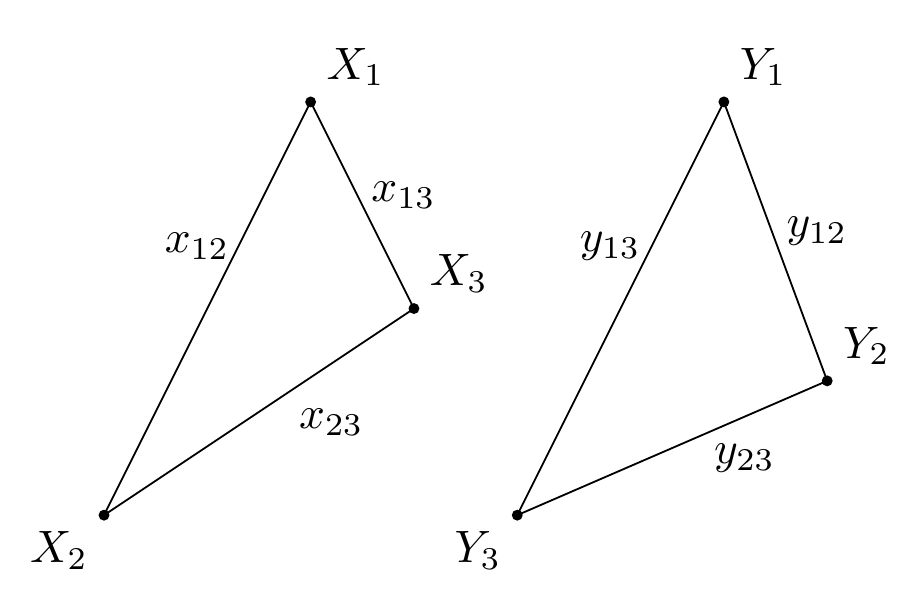
\includegraphics[width=\textwidth]{../simulation/motivating_geometry.png}
		\caption{Geometric structure of source and target samples}
		\label{fig:motivating-geometry}
	\end{subfigure}
	\begin{subfigure}[t]{0.49\textwidth}
		\centering
		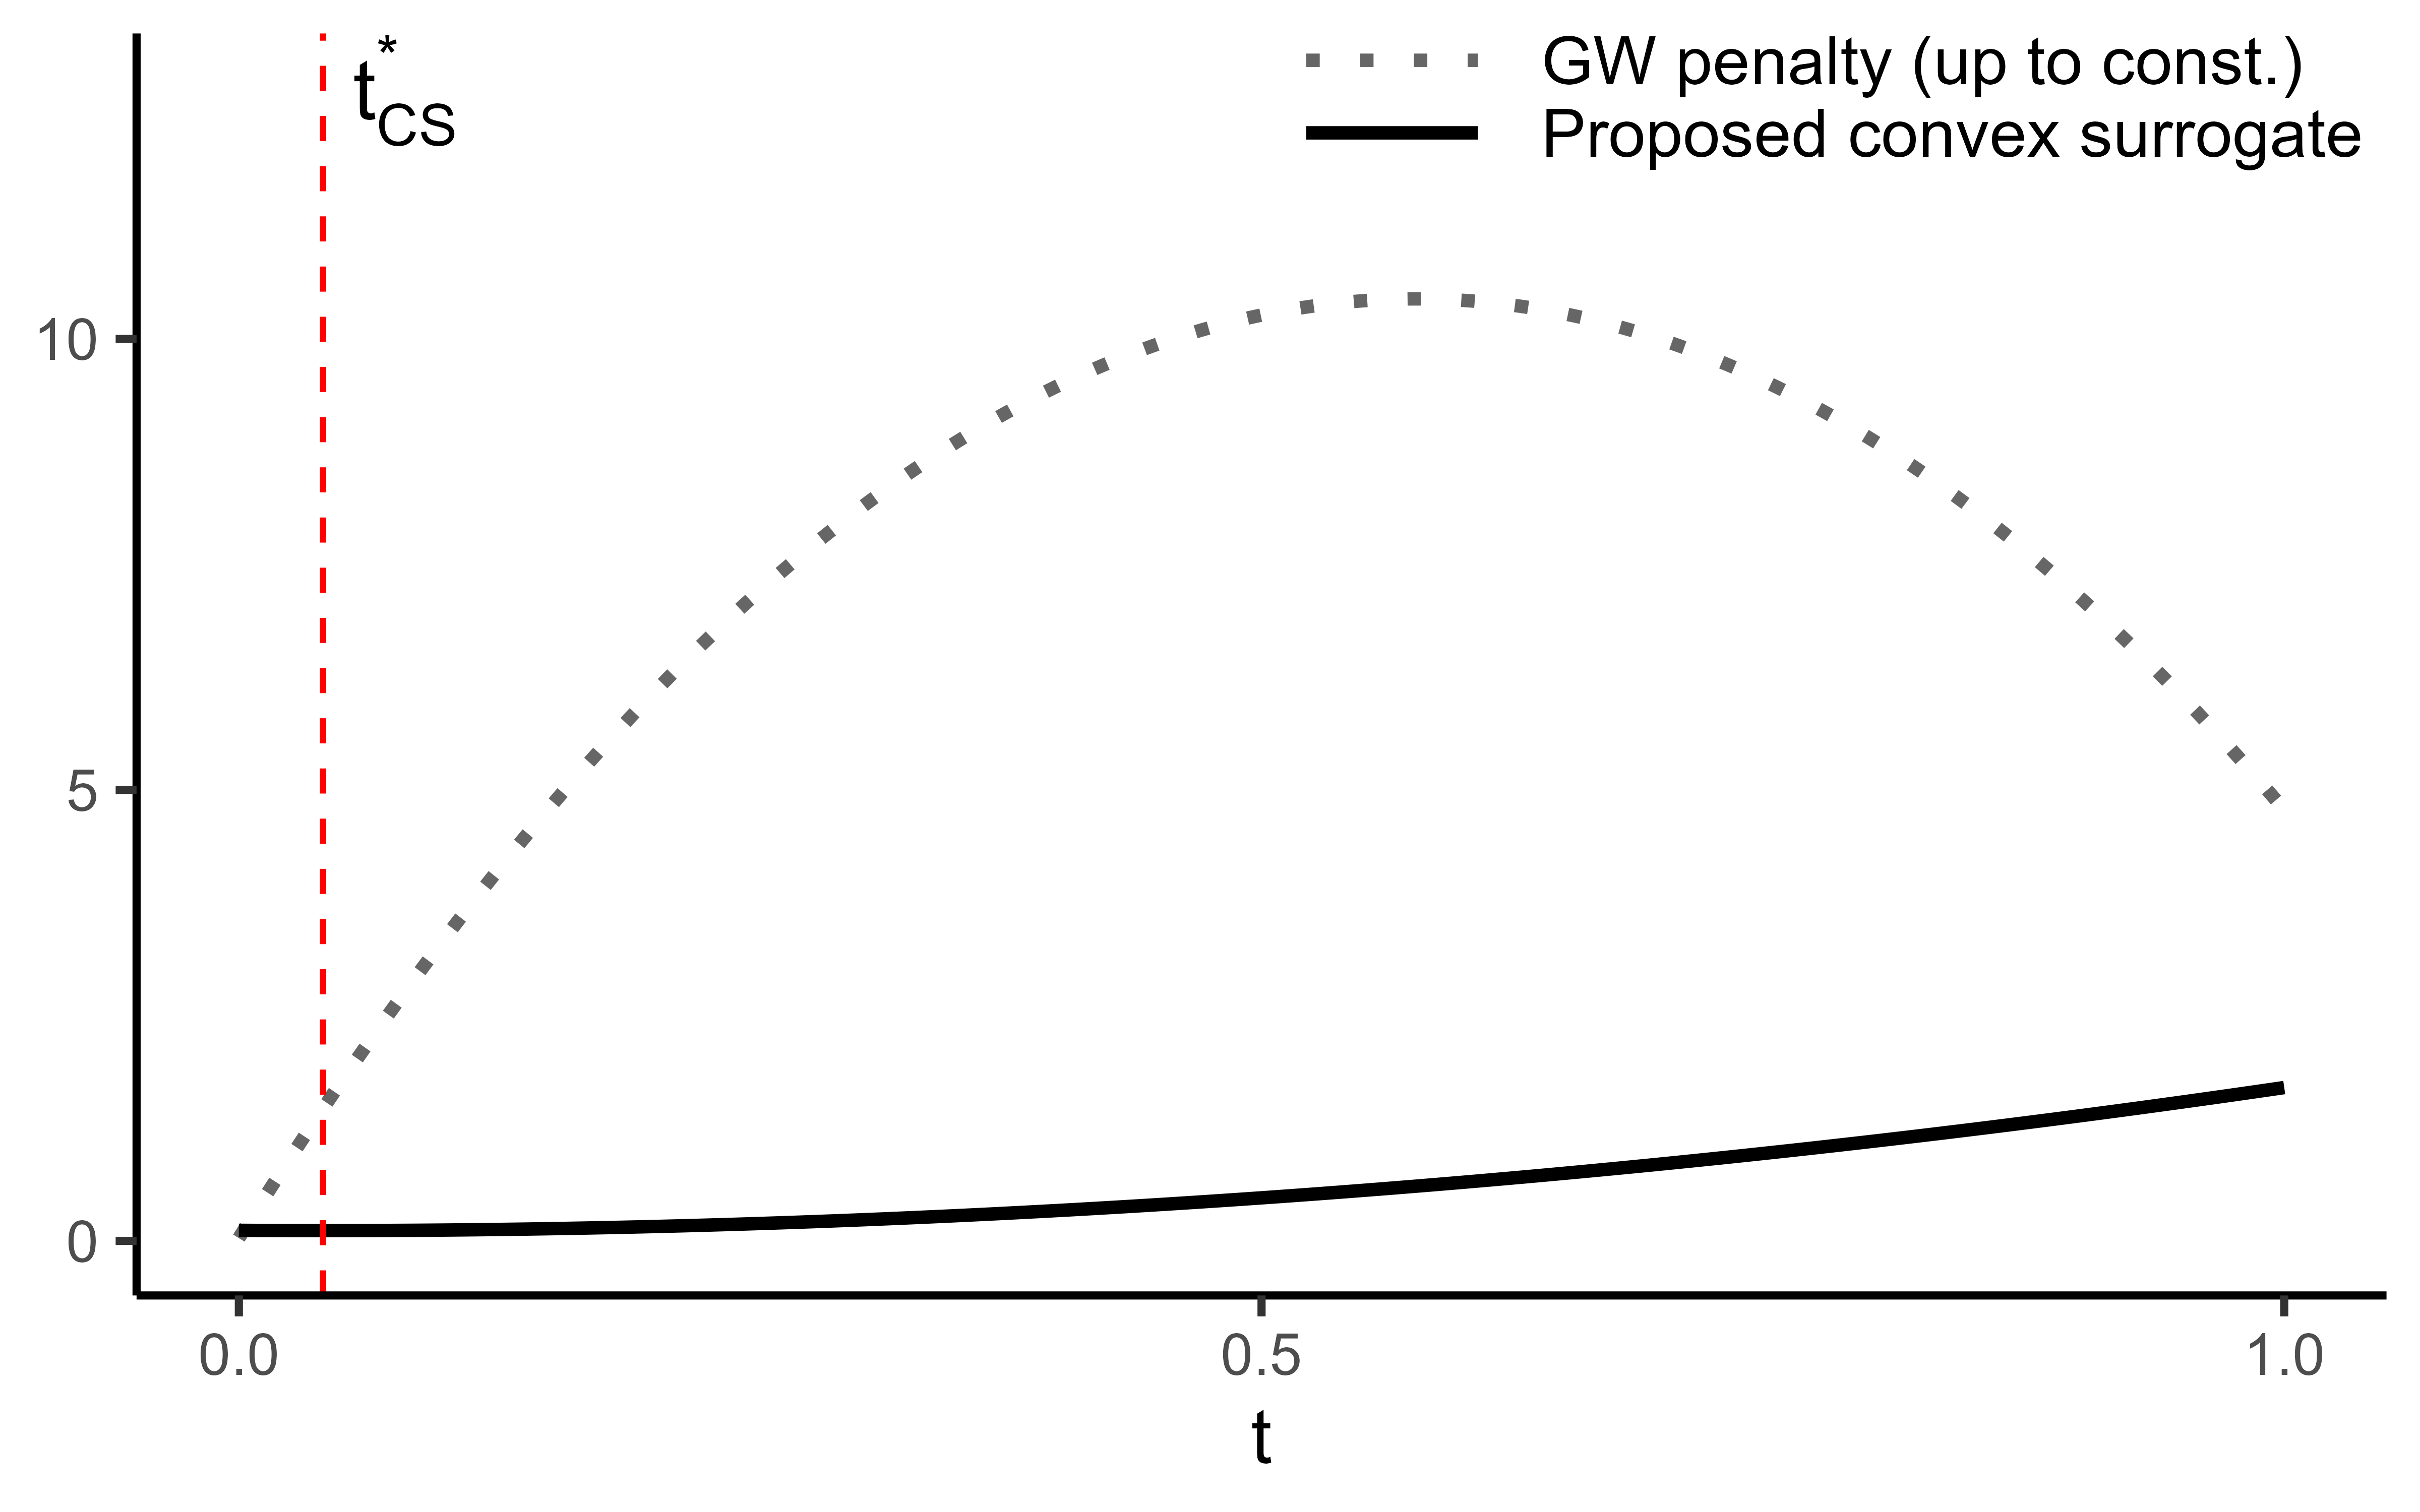
\includegraphics[width=\textwidth]{../simulation/convex_vs_gw.png}
		\caption{Proposed convex surrogate and GW penalty}
		\label{fig:motivating-penalty-trajectory}
	\end{subfigure}
	\caption{Comparison of the geometric structures and associated penalty functions}
	\label{fig:motivating-example}
\end{figure}
%%% Figure explanation: A >> B %%%
Figure~\ref{fig:motivating-example} visualizes the case when $A \gg B \approx 0$. While both penalties encourage small values of $t$, the proposed convex surrogate attains its minimum near zero, whereas the GW penalty reaches its minimum exactly at $t_{\mathrm{GW}}^\ast = 0$. Nevertheless, due to its concave shape, the GW objective may converge to the opposite extreme ($t = 1$) depending on the initialization.

%%% Conclusion %%%
Overall, this example highlights the difference between the proposed convex surrogate and the GW penalty. While the GW objective exhibits a concave behavior that often results in extreme solutions (corresponding to permutation-like transport plans), our convex surrogate yields a smooth and well-behaved solution. In particular, the minimizer $t_{\mathrm{CS}}^\ast$ varies continuously with the geometric discrepancy, while ensuring the convexity. This property ensures numerical stability and uniqueness of the solution, making the convex surrogate more suitable for optimization and statistical analysis, especially in complex settings where the GW 
penalty might fall into suboptimal solutions due to its non-convexity.

\section{Algorithm}\label{sec:Algorithm}
%%% Pseudocode %%%
\begin{algorithm}[t]
	\caption{Convex Quadratic Fused Transport Plan via FW and LAP Projection}
	\label{alg:proposed-algorithm}
	\begin{algorithmic}[1]
		\Require Source data $\{(X_i, f(X_i))\}_{i=1}^{n_X}$, target data $\{(Y_j, f(Y_j))\}_{j=1}^{n_Y}$, weight parameter $0 \leq \alpha \leq 1$, distance kernel $K$, max iters $T$
		
		\State Construct matrices:
		\Statex \hspace{\algorithmicindent} $(C_f)_{ij} \gets \|f(X_i)-f(Y_j)\|_2^2$, \quad
		$(\hat{D}_X^{\kappa})_{ii'} \gets K(X_i,X_{i'})$, \quad
		$(\hat{D}_Y^{\kappa})_{jj'} \gets K(Y_j,Y_{j'})$
		
		\State Initialize $\pi^{(0)} \gets \hat{\mathbb{P}}_X \otimes \hat{\mathbb{P}}_Y$
		
		\For{$t=0,...,T-1$}
		%\State $\nabla F(\pi^{(t)}) \gets C_f + \frac{\lambda}{n_X n_Y}\!\left[A^\top(A\pi^{(t)}-\pi^{(t)}B) - (A\pi^{(t)}-\pi^{(t)}B)B^\top\right]$
		\State Calculate the gradient $\nabla \mathcal{L}_{n_Xn_Y}(\pi^{(t)})$ in \eqref{eq:finite-proposed-method}
		\State Take $\tilde{\pi}^{(t)} \gets \arg\min_{\pi \in \Pi(\hat{\mathbb{P}}_X,\hat{\mathbb{P}}_Y)} \mathrm{Tr}(\nabla \mathcal{L}_{n_Xn_Y}(\pi^{(t)})^\top \pi)$
		\State $\pi^{(t+1)} \gets (1-\gamma_t)\pi^{(t)} + \gamma_t \tilde{\pi}^{(t)}$ for some $0 < \gamma_t < 1$
		\EndFor
		\State $\hat\pi \gets \pi^{(T)}$
		\State \textbf{Optional (LAP):} $\displaystyle
		\hat P \gets \arg\max_{P \in \mathcal{P}} \mathrm{Tr}(P^\top \hat\pi)$, where $\mathcal{P}$ is as defined in \eqref{eq:assign-matrix-space}
		\State \textbf{Return:} $\hat\pi$ (and optionally $\hat P$)
	\end{algorithmic}
\end{algorithm}

%%% Empirical loss %%%
Suppose that we have $(X_i,f(X_i))$ for $i=1,...,n_X$ as source data and $(Y_j,f(Y_j))$ for $j=1,...,n_Y$ as target data. Denote $\hat{\mathbb{P}}_X$ and $\hat{\mathbb{P}}_Y$ by the empirical distributions of $X$ and $Y$, respectively. Then, the empirical version of \eqref{eq:proposed-method} corresponds to
\begin{align*}
	%\label{eq:finite-proposed-method}
	\inf_{\pi \in \Pi(\hat{\mathbb{P}}_X,\hat{\mathbb{P}}_Y)} (1-\alpha)\mathbb{E}_{(X,Y)\sim\pi}\big[\|f(X)-f(Y)\|_2^2\big] + \frac{\alpha}{2} \| D_{\hat{\mathbb{P}}_X}^{\kappa}T_\pi - T_\pi D_{\hat{\mathbb{P}}_Y}^{\kappa} \|_{\mathrm{HS}}^2 .
\end{align*}
In fact, the above problem can be written as a convex quadratic program (and reduces to a linear program when $\alpha = 0$):
\begin{align}
	\label{eq:finite-proposed-method}
	\min_{\pi}\; &\underbrace{(1-\alpha)\mathrm{Tr}\left(C_f^\top \pi\right) + \frac{\alpha}{2n_Xn_Y} \left\| n_Y \hat{D}^{\kappa}_X \pi - n_X \pi \hat{D}^{\kappa}_Y \right\|_F^2}_{\eqqcolon \mathcal{L}_{n_Xn_Y}(\pi)} \nonumber\\
	\mathrm{s.t.}&\quad \pi\mathbf{1}_{n_Y} = \frac{1}{n_X} \mathbf{1}_{n_X} , \quad \pi^\top \mathbf{1}_{n_X} = \frac{1}{n_Y} \mathbf{1}_{n_Y} , \quad \pi \geq 0 ,
\end{align}
where $\pi \in \mathbb{R}_{+}^{n_X \times n_Y}$, $(C_f)_{ij} = \|f(X_i) - f(Y_j)\|_2^2$, $(\hat{D}^{\kappa}_X)_{ii^\prime} = K(X_i,X_{i^\prime})$, and $(\hat{D}^{\kappa}_Y)_{jj^\prime} = K(Y_j,Y_{j^\prime})$.

%%% Optimization algorithm %%%
As \eqref{eq:finite-proposed-method} is a convex quadratic program, numerous standard optimization algorithms are available to find its global minimizer. In this paper, however, we focus on the Frank-Wolfe (FW) algorithm, also known as the conditional gradient (CG) method. The FW algorithm is particularly well-suited for this problem due to its ``projection-free" nature. Unlike projected gradient methods that require a potentially costly projection back onto the feasible set $\Pi(\hat{\mathbb{P}}_X,\hat{\mathbb{P}}_Y)$ at each iteration, the FW algorithm only requires solving a linear minimization problem over this same set. This linear subproblem (or "Linear Minimization Oracle") is often computationally simpler and more efficient to solve than the full projection, making the FW algorithm an attractive choice for optimization problems over the transport polytope.

%%% Find an optimal transport %%%
In many practical applications, it is often more desirable to find a deterministic transport map (or hard assignment) from $X$ to $Y$, rather than the soft coupling $\hat{\pi}$ found by \eqref{eq:finite-proposed-method}. While the optimal solution $\hat{\pi}$ is not guaranteed to be deterministic, we can obtain such a map by solving the following linear assignment problem (LAP):
\begin{align}
	\label{eq:finite-projection-method}
	\hat{P} \coloneqq \argmax_{P \in \mathcal{P}} \mathrm{Tr}(P^\top\hat{\pi}) ,
\end{align}
where $\hat{\pi}$ is an optimal solution to \eqref{eq:finite-proposed-method} and $\mathcal{P}$ denotes the set of deterministic assignment matrices. Specifically, 
\begin{align}
	\label{eq:assign-matrix-space}
	\mathcal{P} \coloneqq \{P \in \{0,1\}^{n_X \times n_Y}: P\mathbf{1}_{n_Y} \leq \mathbf{1}_{n_X}, \; P^\top\mathbf{1}_{n_X} \leq \mathbf{1}_{n_Y}\} .
\end{align}
This LAP seeks the hard assignment $P$ that best aligns with the optimal soft coupling $\hat{\pi}$ and can be solved efficiently using standard methods like the Hungarian algorithm.

%%% Pseudo code description %%%

%%% Computation complexity %%%

%%% Consistency %%%
\paragraph{Consistency}
We first state some technical assumptions to provide a convergence rate for our proposed method.
\begin{assumption}
	\label{ass:consistency}
	$ $
	\begin{itemize}
		\item[(A1)] $(S,d_S,\eta)$ is a $d$-dimensional compact Riemannian manifold.
		\item[(A2)] The densities of $X$ and $Y$, defined by $p_X = d\mathbb{P}_X/d\eta$ and $p_Y = d\mathbb{P}_Y/d\eta$, are strictly bounded above and below:
		\begin{align*}
			0 < p_{\min} \leq p_X,p_Y \leq p_{\max} < \infty .
		\end{align*}
		\item[(A3)] For each $n_X,n_Y \geq 1$, no sample is replicated, that is, all $X_1,...,X_{n_X}$ and $Y_1,...,Y_{n_Y}$ are distinct, respectively.
		%\item[(A4)] $\kappa$ is $L_\kappa$-Lipschitz continuous.
		\item[(A4)] $f$ is $L_f$-Lipschitz continuous.
	\end{itemize}
\end{assumption}

\begin{theorem}
	\label{thm:consistency}
	Let $\hat{\pi}$ be the solution of Algorithm~\ref{alg:proposed-algorithm} with $\alpha > 0$. Suppose that \cref{ass:consistency} holds.
	Then, for some constant $C > 0$,
	\begin{align*}
		\left\vert \mathcal{L}_{n_Xn_Y}(\hat{\pi}) - \inf_{\pi \in \Pi(\mathbb{P}_X,\mathbb{P}_Y)} \mathcal{L}(\pi) \right\vert \leq \underbrace{\frac{8\alpha \, n_{\max}^2}{n_{\min}(T+1)}}_{\text{\emph{Optimization error}}} + C\underbrace{\left(W_2^{d_S}(\mathbb{P}_X,\hat{\mathbb{P}}_X) + W_2^{d_S}(\mathbb{P}_Y,\hat{\mathbb{P}}_Y) \right)}_{\text{\emph{Statistical error}}} .
	\end{align*}
\end{theorem}

%\begin{assumption}[Uniqueness and local quadratic growth]
%	\label{ass:uniqueness-local-quadratic-growth}
%	%	Let $\Pi(\mathbb{P}_X,\mathbb{P}_Y)$ be endowed with the $1$-Wasserstein distance
%	%	$W_1$ on $\mathcal P(S\times S)$ computed with respect to the product metric
%	%	$\bar d((x,y),(x',y')) := d_S(x,x') + d_S(y,y')$.
%	There exists a unique minimizer $\pi^\ast \in \Pi(\mathbb{P}_X,\mathbb{P}_Y)$ of \eqref{eq:proposed-method}. In addition, there exist constants $c>0$ and $\delta>0$ such that
%	\begin{align*}
%		\mathcal{L}(\pi)-\mathcal{L}(\pi^\ast) \;\geq\; c\, W_1(\pi,\pi^\ast)^2 ,
%	\end{align*}
%	for all $\pi\in\Pi(\mathbb{P}_X,\mathbb{P}_Y)$ with $\mathcal{L}(\pi)\le \mathcal{L}(\pi^\ast)+\delta$.
%\end{assumption}
%
%\begin{corollary}
%	Let $\hat{\pi}$ be the solution of Algorithm~\ref{alg:proposed-algorithm} with $\alpha > 0$. Suppose that \cref{ass:uniqueness-local-quadratic-growth} holds. For any $0 < \varepsilon < \sqrt{\delta/c}$, choose the maximum number of iteration $T$ as
%	\begin{align*}
%		T + 1 \geq \frac{24\alpha(\sup\kappa)^2}{c\varepsilon^2 h^2} \cdot \frac{n_{\max}^2}{n_{\min}} .
%	\end{align*}
%	Then,
%	\begin{align*}
%		\mathbb{P}\left(W_1(\hat{\pi},\pi^\ast) > \varepsilon \right) \leq ...
%	\end{align*}
%\end{corollary}

\section{Numerical Experiments}\label{sec:Experiments}
%%% Intro %%%
This section provides numerical experiments to empirically validate the main results: (i) the proposed algorithm asymptotically returns a global minimizer of \eqref{eq:proposed-method}; and (ii) it provides a compelling estimator that strikes a balance between minimizing transport costs in feature space and preserving geometry.

\subsection{Empirical Evidence}

\subsection{Comparison to FGW Method}
In this section, we aim to demonstrate the performance of our proposed algorithm~\eqref{eq:proposed-method} compared to the FGW method~\eqref{eq:pi-fused-ot} with graph data.

\paragraph{Data generation.}
%%% Structure %%%
We conduct a simulation study generating $100$ instances of lattice-structured objects with clusters. Each simulated instance consists of an undirected graph with $B \in \{2,3,4\}$ latent blocks and $N \in \{B^3, B^5, B^7\}$ nodes.
To generate ground-truth correspondences with controlled structural similarity, we first sample a lattice block model whose within-block connectivity is organized as a two-dimensional grid.
Specifically, nodes within each block are arranged on a nearly square lattice and connected via von Neumann (4-neighbor) wiring, while edges between different blocks are added independently with probability $p_{\text{out}} = 0.02$.

%%% Target generation %%%
To construct the paired graphs $(G_X, G_Y)$, we first generate $G_X$ from the above model, and then apply a block-wise permutation $P_{\text{true}}$ that shuffles node identities within each block and permutes the block order according to
\begin{align*}
	b_{\text{target}} \equiv b_{\text{source}} + 1 \pmod B .
\end{align*}
The resulting $G_Y = P_{\text{true}}^\top G_X P_{\text{true}}$ thus represents an isomorphism of $G_X$ but with latent correspondences obscured both within and across blocks. Figure~\ref{fig:data-example} shows an example for simulated lattice block models used in the experiments.

%%% Feature %%%
Each node $i$ is further assigned a feature vector $f_i \in \mathbb{R}^B$ drawn from a $B$-dimensional Gaussian aligned with the block labels: if node $i$ belongs to the $b$-th cluster,
\begin{align*}
	f(i) \sim N(e_b,\sigma^2 I_B) , \quad e_b = [0,...0,\underset{\text{$b$-th}}{1},0,...,0]^\top ,
\end{align*}
where $\sigma^2 \in \{0,0.001,1\}$, so that features are discriminative at the block level but nearly indistinguishable within each block, especially when $\sigma^2$ is small.

\begin{figure}[t]
	\centering
	\begin{subfigure}{\textwidth}
		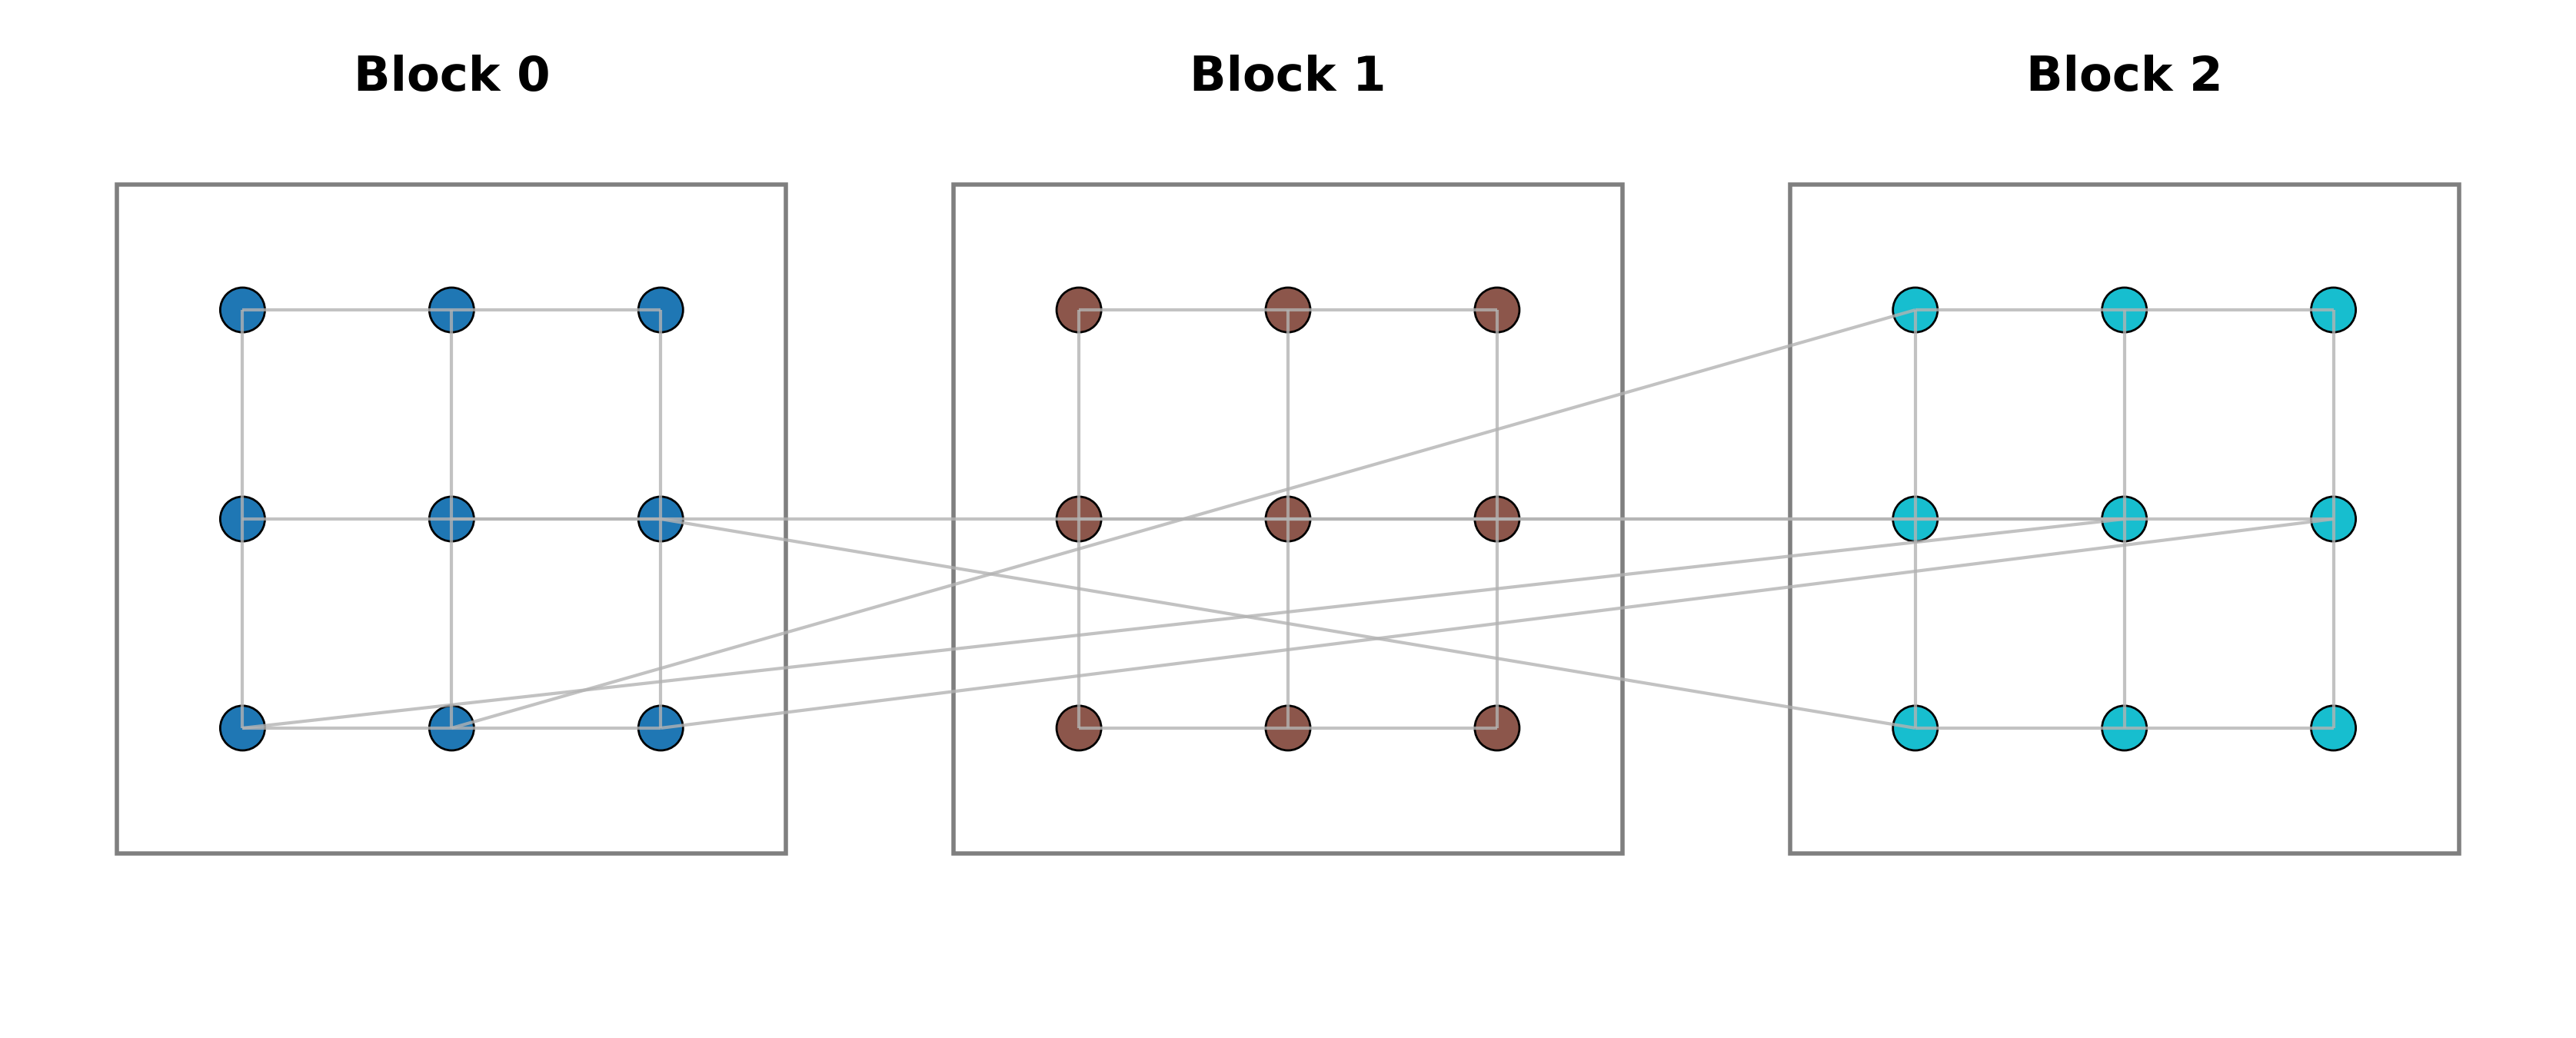
\includegraphics[width=\textwidth]{../simulation/source_lattice_blocks.png}
		\caption{Source graph $G_X$ consisting of three lattice-structured blocks ($B=3$, $N=27$).}
		\label{fig:data-example-source}
	\end{subfigure}
	\begin{subfigure}{\textwidth}
		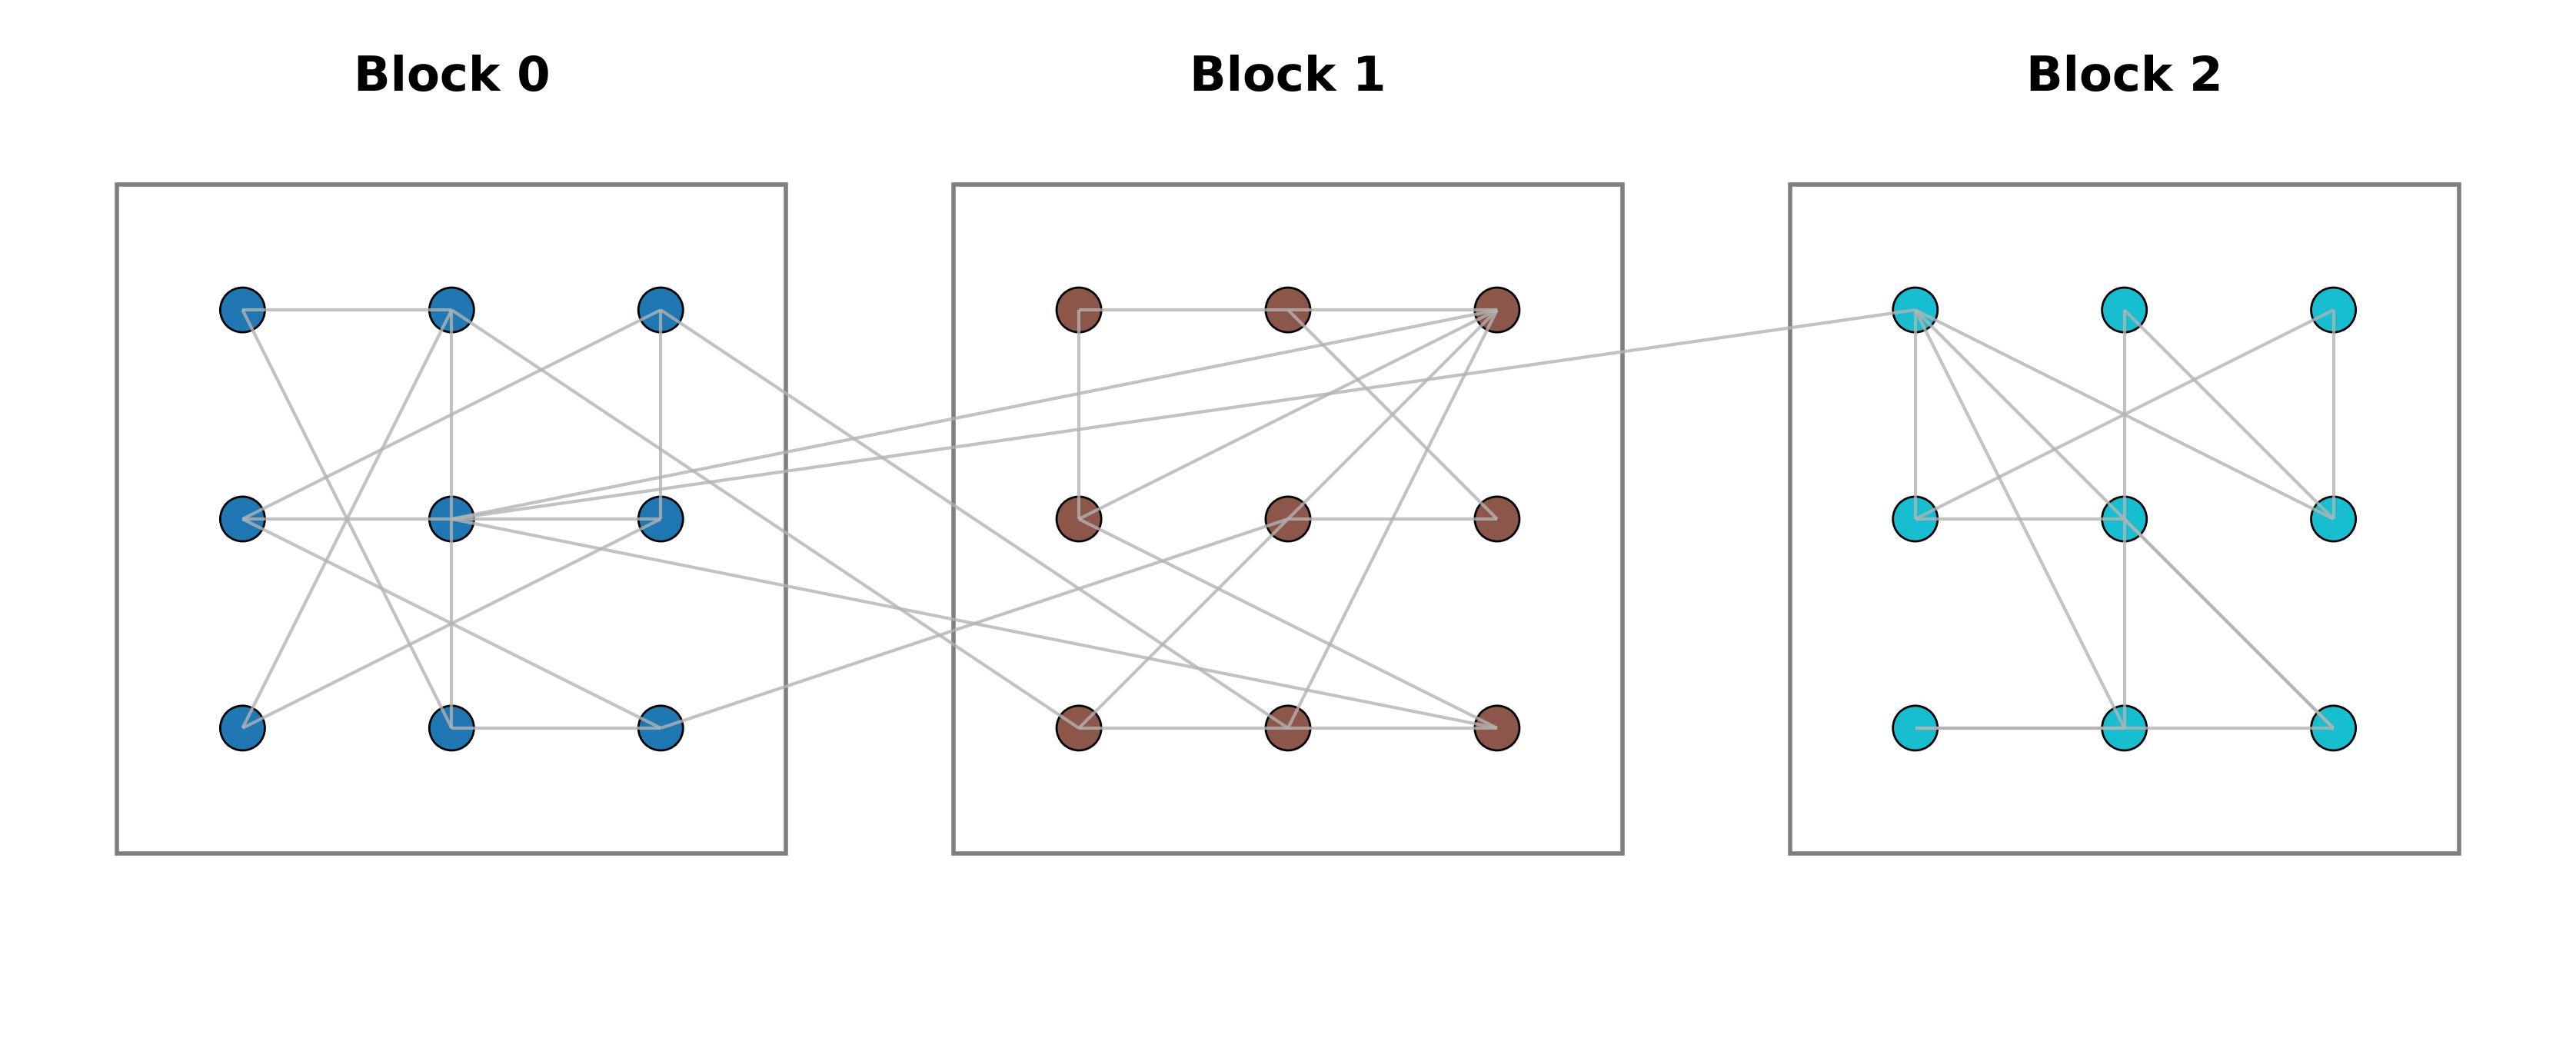
\includegraphics[width=\textwidth]{../simulation/target_lattice_blocks.png}
		\caption{Target graph $G_Y$ obtained by applying a within-block shuffling and a cyclic block permutation to $G_X$.}
		\label{fig:data-example-target}
	\end{subfigure}
	\caption{Illustration of simulated lattice block models. The target graph preserves the same global structure as the source but obscures node-wise correspondences both within and across blocks.}
	\label{fig:data-example}
\end{figure}

\paragraph{Implementation details.}
The pairwise feature cost is defined by the squared Euclidean distance $C_f(i,j) = \|f(i) - f(j)\|_2^2$, as specified in Algorithm~\ref{alg:proposed-algorithm}. To encode structural geometry, we employ two complementary metrics: the geodesic distance and the heat kernel. 

%%% Geodesic distance %%%
The geodesic distance between nodes $i$ and $j$ is defined as the length of the shortest path connecting them:
\begin{align*}
	d_{G}(i,j) \coloneqq \min_{\xi: i \leadsto j} |\xi| ,
\end{align*}
where $\xi : i \leadsto j$ denotes a path from $i$ to $j$, and $|\xi|$ denotes the number of edges contained in that path. For the geodesic distance, we use a standard Gaussian kernel $\kappa(x) = \exp(-x^2)$, i.e., $K_G(i,j) = \exp(-d_G(i,j)^2)$.

%%% Heat kernel %%%
The heat kernel provides a smooth diffusion-based measure of proximity that captures multi-scale structural relationships. Given the graph Laplacian $L = D - G$, where $G \in \{0,1\}^{n \times n}$ is the adjacency matrix and $D = \mathrm{diag}(G \mathbf{1}_n)$ is the degree matrix, 
the heat kernel at time scale $t > 0$ is defined by
\begin{align*}
	K_t \coloneqq e^{-tL} ,
\end{align*}
so that $K_H(i,j ; t) \coloneqq [K_t]_{ij}$ represents the amount of heat transferred from node $i$ to node $j$ after diffusion time $t$. In our experiments, we fix at $t=1$.
In practice, $K_t$ can be efficiently approximated by a second order Taylor expansion:
\begin{align*}
	K_t \approx I - tL + \tfrac{1}{2}t^2L^2 ,
\end{align*}
which preserves locality while maintaining computational tractability. We should note that the heat kernel is not a distance; however, it is widely used in practice as a similarity measure that reflects both local connectivity and global diffusion properties of the graph. Compared to the geodesic distance, which captures discrete shortest-path relations, the heat kernel encodes continuous multi-scale interactions between nodes and is particularly effective for capturing smooth structural correspondences.

%%% Hyperparameter %%%
The following outlines the hyperparameter and implementation settings used throughout our experiments. For the weight parameter, we set $\alpha \in \{0,0.25,0.5,0.75,1\}$ for both methods. 
We fix the number of iterations at $T=100$ across all settings. We report performance based on the estimator $\hat{P}$, and, for comparison, we use the \texttt{gromov.fused\_gromov\_wasserstein} function provided in the \texttt{POT} library (Python) to implement the FGW method.


%%% References %%%
\bibliographystyle{abbrvnat}
\bibliography{FOT_references}


%%%%%%%%%%%%%%%%%%%%%%%%%%%%%%%%%%%%%%%%%%%%%%%%%%%          %%%%%%%%%%%%%%%%%%%%%%%%%%%%%%%%%%%%%%%%%%%%%%%%%%%
%%%%%%%%%%%%%%%%%%%%%%%%%%%%%%%%%%%%%%%%%%%%%%%%%%% Appendix %%%%%%%%%%%%%%%%%%%%%%%%%%%%%%%%%%%%%%%%%%%%%%%%%%%
%%%%%%%%%%%%%%%%%%%%%%%%%%%%%%%%%%%%%%%%%%%%%%%%%%%          %%%%%%%%%%%%%%%%%%%%%%%%%%%%%%%%%%%%%%%%%%%%%%%%%%%

\appendix
\section{Appendix}
\subsection{Proof for \cref{lem:regularization-term}}\label{pf:lem:regularization-term}
\begin{proof}
	For $g \in L^2(S,\mathbb{P}_Y)$, observe that
	\begin{align*}
		&(D_{\mathbb{P}_X}^{\kappa}T_{\pi}g)(x) = \mathbb{E}\Big[K(x,X)\mathbb{E}\left[g(Y) \mid X\right]\Big] = \int_S \Gamma_\pi^1(x,y)g(y)\mathbb{P}_Y(dy) , \\
		&(T_{\pi}D_{\mathbb{P}_Y}^{\kappa}g)(x) = \mathbb{E}\Big[(D_{\mathbb{P}_Y}^{\kappa}g)(Y) \mid X = x\Big] = \int_S \Gamma_\pi^2(x,y)g(y) \mathbb{P}_Y(dy) .
	\end{align*}
	Since $K$ is bounded, $D_{\mathbb{P}_X}^{\kappa}T_{\pi} - T_{\pi}D_{\mathbb{P}_Y}^{\kappa}$ is a well-defined Hilbert-Schmidt operator with a kernel $\Gamma_\pi(x,y)$:
	\begin{align*}
		\| D_{\mathbb{P}_X}^{\kappa}T_{\pi} - T_{\pi}D_{\mathbb{P}_Y}^{\kappa} \|_{\mathrm{HS}}^2 = \int_S\int_S \Gamma_\pi(x,y)^2\mathbb{P}_X(dx)\mathbb{P}_Y(dy) \leq 4 .
	\end{align*}
\end{proof}

\subsection{Proof for \cref{thm:convex-relaxation}}\label{pf:thm:convex-relaxation}
\begin{proof}
	Refer to \cref{lem:regularization-term} to confirm that the operator $D_{\mathbb{P}_X}^{\kappa}T_{\pi} - T_{\pi}D_{\mathbb{P}_Y}^{\kappa}$ is well-defined and Hilbert--Schmidt for any $\pi \in \Pi(\mathbb{P}_X,\mathbb{P}_Y)$. 
	To establish convexity of \eqref{eq:proposed-method}, it suffices to show that 
	\begin{align*}
	\pi \;\mapsto\; \|D_{\mathbb{P}_X}^{\kappa}T_\pi - T_\pi D_{\mathbb{P}_Y}^{\kappa}\|_{\mathrm{HS}}^2
	\end{align*}
	is convex on $\Pi(\mathbb{P}_X,\mathbb{P}_Y)$.
	
	Let $\pi_1,\pi_2 \in \Pi(\mathbb{P}_X,\mathbb{P}_Y)$ and $t \in [0,1]$, and define $\pi_t = t\pi_1 + (1-t)\pi_2$. 
	Since both $\pi_1$ and $\pi_2$ share the same marginals $\mathbb{P}_X$ and $\mathbb{P}_Y$, 
	the disintegration theorem ensures that their corresponding conditional kernels satisfy
	\begin{align*}
	k_t(\cdot|x) = t\,k_1(\cdot|x) + (1-t)\,k_2(\cdot|x)
	\quad \text{for} \;\; \mathbb{P}_X\text{-a.e.} \; x \in S.
	\end{align*}
	That is, the conditional distribution of $Y$ given $X=x$ under $\pi_t$ is the convex combination of the conditional distributions under $\pi_1$ and $\pi_2$. 
	Consequently, for any $g \in L^2(S,\mathbb{P}_Y)$,
	\begin{align*}
		(T_{\pi_t} g)(x)
		&= \int g(y)\,k_t(dy|x)
		= t \int g(y)\,k_1(dy|x) + (1-t)\int g(y)\,k_2(dy|x) \\
		&= t\,(T_{\pi_1}g)(x) + (1-t)\,(T_{\pi_2}g)(x),
	\end{align*}
	which shows that $T_{\pi_t}$ depends affinely on $\pi$, i.e.,
	\begin{align*}
	T_{\pi_t} = t\,T_{\pi_1} + (1-t)\,T_{\pi_2}.
	\end{align*}
	
	Because $D_{\mathbb{P}_X}^{\kappa}$ and $D_{\mathbb{P}_Y}^{\kappa}$ are linear operators, it follows that
	\begin{align*}
	D_{\mathbb{P}_X}^{\kappa}T_{\pi_t} - T_{\pi_t}D_{\mathbb{P}_Y}^{\kappa}
	= t\,(D_{\mathbb{P}_X}^{\kappa}T_{\pi_1} - T_{\pi_1}D_{\mathbb{P}_Y}^{\kappa})
	+ (1-t)\,(D_{\mathbb{P}_X}^{\kappa}T_{\pi_2} - T_{\pi_2}D_{\mathbb{P}_Y}^{\kappa}).
	\end{align*}
	Denoting $A_i := D_{\mathbb{P}_X}^{\kappa}T_{\pi_i} - T_{\pi_i}D_{\mathbb{P}_Y}^{\kappa}$ $(i=1,2)$ and $A_t := D_{\mathbb{P}_X}^{\kappa}T_{\pi_t} - T_{\pi_t}D_{\mathbb{P}_Y}^{\kappa}$, 
	we have $A_t = tA_1 + (1-t)A_2$. 
	Since $\|\cdot\|_{\mathrm{HS}}^2$ is convex, we obtain
	\begin{align*}
	\|A_t\|_{\mathrm{HS}}^2
	= \|tA_1 + (1-t)A_2\|_{\mathrm{HS}}^2
	\le t\,\|A_1\|_{\mathrm{HS}}^2 + (1-t)\,\|A_2\|_{\mathrm{HS}}^2.
	\end{align*}
	Therefore, $\pi \mapsto \|D_{\mathbb{P}_X}^{\kappa}T_\pi - T_\pi D_{\mathbb{P}_Y}^{\kappa}\|_{\mathrm{HS}}^2$ is convex on $\Pi(\mathbb{P}_X,\mathbb{P}_Y)$. 
\end{proof}

\subsection{Proof for \cref{prop:solution}}\label{pf:prop:solution}
\begin{proof}
	Since $Y = T(X)$ almost surely, for any $(x,y) \in \mathrm{supp}(\pi)$, we have
	\begin{align*}
		\Gamma_\pi^1(x,y) &= \mathbb{E}[K(x,X)\mid Y=y] = \kappa\left(d_S\bigl(x,T^{-1}(y)\bigr)\right), \\
		\Gamma_\pi^2(x,y) &= \mathbb{E}[K(y,Y)\mid X=x] = \kappa\left(d_S\bigl(y,T(x)\bigr)\right).
	\end{align*}
	Hence, for such $(x,y)$,
	\begin{align*}
		\Gamma_\pi(x,y)
		= \Gamma_\pi^1(x,y) - \Gamma_\pi^2(x,y)
		= \kappa\left(d_S\bigl(x,T^{-1}(y)\bigr)\right) - \kappa\left(d_S\bigl(y,T(x)\bigr)\right) .
	\end{align*}
	Now, setting $y = T(x')$ gives
	\begin{align*}
		\Gamma_\pi\bigl(x,T(x')\bigr)
		= \kappa\left(d_S\bigl(x,x^\prime\bigr)\right) - \kappa\left(d_S\bigl(T(x),T(x^\prime)\bigr)\right) .
	\end{align*}
	
	($\Leftarrow$) If $d_S(T(x),T(x')) = d_S(x,x')$ holds for $\mathbb{P}_X \otimes \mathbb{P}_X$-almost every $(x,x')$, substituting this into the above expression yields $\Gamma_\pi(x,T(x')) = 0$ for $\mathbb{P}_X \otimes \mathbb{P}_X$-almost every $(x,x')$. Consequently, $\Gamma_\pi = 0$ holds for $\pi$-almost every $(x,y)$, which implies that the Hilbert–Schmidt norm is zero.
	
	($\Rightarrow$) Now, assume that $\kappa$ is strictly monotone. If $\|D_{\mathbb{P}_X}^{\kappa}T_\pi - T_\pi D_{\mathbb{P}_Y}^{\kappa}\|_{\mathrm{HS}}^2 = 0$, then $\Gamma_\pi = 0$ holds for $\mathbb{P}_X \otimes \mathbb{P}_Y$-almost every $(x,y)$, and in particular, for pairs $(x,T(x'))$ with respect to $\mathbb{P}_X \otimes \mathbb{P}_X$-almost every $(x,x')$. By the strict monotone property of $\kappa$, $d_S(T(x),T(x^\prime)) = d_S(x,x^\prime)$ holds for $\mathbb{P}_X \otimes \mathbb{P}_X$-almost every $(x,x^\prime)$.
	
	Finally, if $T$ is continuous and $\mathrm{supp}(\mathbb{P}_X) = S$, then the function
	\begin{align*}
		F(x,x') := K(x,x') - K(T(x),T(x'))
	\end{align*}
	is continuous and vanishes on the dense set $\mathrm{supp}(\mathbb{P}_X) \times \mathrm{supp}(\mathbb{P}_X)$.  
	By continuity, $F \equiv 0$ on $S \times S$.
	Again by the strict monotonicity of $\kappa$, $d_S(T(x),T(x')) = d_S(x,x')$ holds for all $x,x' \in S$, implying that $T$ is an isometry on $S$.
\end{proof}

\subsection{Proof for \cref{thm:consistency}}\label{pf:thm:consistency}
\begin{proof}
	One key of consistency is to calculate the convergence rate of empirical distributions. To this end, we first introduce the Wasserstein-$1$ distance.
	\begin{definition}[Wasserstein-$p$ distance]
		\label{def:Wasserstein-p}
		Let $(S,d_S)$ be a compact metric space. For probability measures $\mu$ and $\nu$ on $S$, we define
		\begin{align*}
			W_p^S(\mu,\nu) \coloneqq \inf_{\pi \in \Pi(\mu,\nu)} \left(\int_{S \times S} d_S(x,y)^p \pi(dx,dy)\right)^{1/p} . 
		\end{align*}
	\end{definition}
	
	\begin{lemma}
		\label{lem:equivalence-to-weak-convergence}
		Consider the sequence of probability measures $\{\mu_n: n \geq 1\}$ and $\mu$ on $S$. Then,
		\begin{align*}
			W_p^S(\mu_n,\mu) \to 0 \;\; \text{as} \;\; n \to \infty \iff \mu_n \overset{w}{\to} \mu \;\; \text{as} \;\; n \to \infty ,
		\end{align*}
		where $\mu_n \overset{w}{\to} \mu$ denotes the weak convergence.
	\end{lemma}
	\begin{proof}
		See details in \cite{villani2008optimal}.
	\end{proof}
	
	First, note that
	\begin{align*}
		&\left\vert \mathcal{L}_{n_Xn_Y}(\hat{\pi}) - \inf_{\pi \in \Pi(\mathbb{P}_X,\mathbb{P}_Y)} \mathcal{L}(\pi) \right\vert \\
		&\leq \left\vert \mathcal{L}_{n_Xn_Y}(\hat{\pi}) - \inf_{\pi \in \Pi(\hat{\mathbb{P}}_X,\hat{\mathbb{P}}_Y)} \mathcal{L}_{n_Xn_Y}(\pi) \right\vert + \left\vert \inf_{\pi \in \Pi(\hat{\mathbb{P}}_X,\hat{\mathbb{P}}_Y)} \mathcal{L}_{n_Xn_Y}(\pi) - \inf_{\pi \in \Pi(\mathbb{P}_X,\mathbb{P}_Y)} \mathcal{L}(\pi) \right\vert \\
		&\eqqcolon E_1 + E_2 .
	\end{align*}
	
	%%% Optimization error %%%
	We first provide the bound for $E_1$, which is the optimization error.
%	\begin{lemma}
%		\label{lem:smooth-loss}
%		For all $n_X,n_Y \geq 1$ and $\pi_1,\pi_2 \in \Pi(\hat{\mathbb{P}}_X,\hat{\mathbb{P}}_Y)$,
%		\begin{align*}
%			\Big\| \nabla \mathcal{L}_{n_Xn_Y}(\pi_1) - \nabla \mathcal{L}_{n_Xn_Y}(\pi_2) \Big\|_F \leq \alpha \cdot \frac{n_{\max}}{n_{\min}} \left(\|D_{\hat{\mathbb{P}}_X}^\kappa\|_{\mathrm{op}} + \|D_{\hat{\mathbb{P}}_Y}^\kappa\|_{\mathrm{op}}\right)^2 \|\pi_1 - \pi_2\|_F .
%		\end{align*} 
%	\end{lemma}
%	\begin{proof}
%		See Appendix~\ref{pf:lem:smooth-loss}.
%	\end{proof}
%	\cref{lem:smooth-loss} guarantees the smoothness of $\mathcal{L}_{n_Xn_Y}$.
	
	\begin{lemma}
		\label{lem:FW-convergence}
		Let $\{\pi^{(t)}: t \geq 0\}$ be the sequence of iterates generated by Algorithm~\ref{alg:proposed-algorithm} with
		\begin{align*}
			\gamma_t = \frac{2}{t+2} ,
		\end{align*}
		for each $t$. Then, for any $t \geq 1$,
		\begin{align*}
			\mathcal{L}_{n_Xn_Y}(\pi^{(t)}) - \inf\mathcal{L}_{n_Xn_Y} \leq \frac{2\alpha}{n_{\min}(t+1)} \left(\|\hat{D}_X^\kappa\|_{\mathrm{op}} + \|\hat{D}_Y^\kappa\|_{\mathrm{op}}\right)^2 .
		\end{align*}
	\end{lemma}
	\begin{proof}
		See Appendix~\ref{pf:lem:FW-convergence}.
	\end{proof}
	
	The proof for \cref{lem:FW-convergence} is a standard technique to show the convergence of the FW algorithm. Considering that $\|\cdot\|_{\mathrm{op}} \leq \|\cdot\|_{\infty}$,
	\begin{align*}
		\|\hat{D}_X^\kappa\|_{\mathrm{op}} \leq \max_{i} \sum_{j=1}^{n_X} [\hat{D}_X^\kappa]_{ij} \leq n_X , \quad \|\hat{D}_Y^\kappa\|_{\mathrm{op}} \leq n_Y .
	\end{align*}
	This gives that
	\begin{align*}
		\left(\|\hat{D}_X^\kappa\|_{\mathrm{op}} + \|\hat{D}_Y^\kappa\|_{\mathrm{op}}\right)^2 \leq 4n_{\max}^2 .
	\end{align*}
	Thus,
	\begin{align*}
		E_1 \leq \frac{8\alpha \, n_{\max}^2}{n_{\min}(T+1)} .
	\end{align*}
	
	To control the bound of $E_2$, we introduce a useful lemma known as the gluing lemma.
	\begin{lemma}[Gluing lemma]
		Let $(\mathcal{X}_i,\mu_i)$, $i=1,2,3$, be Polish probability spaces. If $(X_1,X_2)$ is a coupling of $(\mu_1,\mu_2)$ and $(Y_2,Y_3)$ is a coupling of $(\mu_2,\mu_3)$, then one can construct a triple of random elements $(Z_1,Z_2,Z_3)$ such that $(Z_1,Z_2)$ has the same distribution as $(X_1,X_2)$ and $(Z_2,Z_3)$ has the same distribution as $(Y_2,Y_3)$.
	\end{lemma}
	\begin{proof}
		See details in \cite{villani2008optimal}.
	\end{proof}
	To use the gluing lemma, we first define two projection couplings $Q_X \in \Pi(\mathbb{P}_X,\hat{\mathbb{P}}_X)$ and $Q_Y \in \Pi(\hat{\mathbb{P}}_Y,\mathbb{P}_Y)$, which will be specified later.
%	\begin{align*}
%		Q_X \in \argmin_{\pi \in \Pi(\mathbb{P}_X,\hat{\mathbb{P}}_X)} \mathbb{E}_{(X,\hat{X}) \sim Q}\left[d_S(X,\hat{X})\right] , \quad Q_Y \in \argmin_{\pi \in \Pi(\hat{\mathbb{P}}_Y,\mathbb{P}_Y)} \mathbb{E}_{(\hat{Y},Y) \sim Q}\left[d_S(\hat{Y},Y)\right] .
%	\end{align*}
%	Then, by \cref{def:Wasserstein-1}, we get
%	\begin{align*}
%		&W_1(\mathbb{P}_X,\hat{\mathbb{P}}_X) = \mathbb{E}_{(X,\hat{X}) \sim Q_X} \left[d_S(X,\hat{X})\right] , \\
%		&W_1(\hat{\mathbb{P}}_Y,\mathbb{P}_Y) = \mathbb{E}_{(\hat{Y},Y) \sim Q_Y}\left[d_S(\hat{Y},Y)\right] .
%	\end{align*} 
	
	For an arbitrary $\pi \in \Pi(\hat{\mathbb{P}}_X,\hat{\mathbb{P}}_Y)$, we can construct a coupling $\Xi \in \Pi(\mathbb{P}_X,\hat{\mathbb{P}}_X,\hat{\mathbb{P}}_Y,\mathbb{P}_Y)$ such that
	\begin{align}
		\label{eq:glued-coupling}
		\Xi(dx,d\hat{x},d\hat{y},dy) = \underbrace{Q_Y(dy \mid \hat{y})}_{\hat{\mathbb{P}}_Y \to \mathbb{P}_Y} \; \underbrace{\pi(d\hat{y} \mid \hat{x})}_{\hat{\mathbb{P}}_X \to \hat{\mathbb{P}}_Y} \; \underbrace{Q_X(dx \mid \hat{x})}_{\hat{\mathbb{P}}_X \to \mathbb{P}_X} \; \hat{\mathbb{P}}_X(d\hat{x}) ,
	\end{align}
	owing to the gluing lemma. Then, define
	\begin{align*}
		\Phi_n(\pi)(dx,dy) \coloneqq \int_{(\hat{x},\hat{y}) \in S \times S}  Q_X(dx \mid \hat{x}) \; Q_Y(dy \mid \hat{y}) \; \pi(d\hat{y} \mid \hat{x}) \; \hat{\mathbb{P}}_X(d\hat{x}) ,
	\end{align*}
	which makes clear that $\Phi_n(\pi) : \Pi(\hat{\mathbb{P}}_X,\hat{\mathbb{P}}_Y) \to \Pi(\mathbb{P}_X,\mathbb{P}_Y)$ is a well-defined function that maps the coupling on $\Pi(\hat{\mathbb{P}}_X,\hat{\mathbb{P}}_Y)$ to that on $\Pi(\mathbb{P}_X,\mathbb{P}_Y)$.
	
	Let $\pi^\ast_n \in \argmin_{\pi \in \Pi(\hat{\mathbb{P}}_X,\hat{\mathbb{P}}_Y)} \mathcal{L}_{n_Xn_Y}(\pi)$. Observe that
	\begin{align*}
		&\left\vert \mathcal{L}_{n_Xn_Y}(\pi^\ast_n) - \inf_{\pi \in \Pi(\mathbb{P}_X,\mathbb{P}_Y)} \mathcal{L}(\pi) \right\vert \\
		&\leq \left\vert \mathcal{L}_{n_Xn_Y}(\pi^\ast_n) - \mathcal{L}(\Phi_n(\pi^\ast_n)) \right\vert + \left\vert \mathcal{L}(\Phi_n(\pi^\ast_n)) - \inf_{\pi \in \Pi(\mathbb{P}_X,\mathbb{P}_Y)} \mathcal{L}(\pi) \right\vert \\[5pt]
		&\leq \sup_{\pi \in \Pi(\hat{\mathbb{P}}_X,\hat{\mathbb{P}}_Y)} \left\vert \mathcal{L}_{n_Xn_Y}(\pi) - \mathcal{L}(\Phi_n(\pi)) \right\vert \\
		&\qquad\qquad\qquad + \left\vert \mathcal{L}(\Phi_n(\pi^\ast_n)) -  \mathcal{L}_{n_Xn_Y}(\pi^\ast_n) \right\vert + \left\vert \mathcal{L}_{n_Xn_Y}(\pi^\ast_n) - \inf_{\pi \in \Pi(\hat{\mathbb{P}}_X,\hat{\mathbb{P}}_Y)} \mathcal{L}(\Phi_n(\pi)) \right\vert \\
		&\qquad\qquad\qquad\qquad\qquad\qquad\qquad\qquad\qquad\qquad + \left\vert \inf_{\pi \in \Pi(\hat{\mathbb{P}}_X,\hat{\mathbb{P}}_Y)} \mathcal{L}(\Phi_n(\pi)) - \inf_{\pi \in \Pi(\mathbb{P}_X,\mathbb{P}_Y)} \mathcal{L}(\pi) \right\vert \\
		&\leq 3\underbrace{\sup_{\pi \in \Pi(\hat{\mathbb{P}}_X,\hat{\mathbb{P}}_Y)} \left\vert \mathcal{L}_{n_Xn_Y}(\pi) - \mathcal{L}(\Phi_n(\pi)) \right\vert}_{\eqqcolon \mathrm{I}_n} + \underbrace{\left\vert \inf_{\pi \in \Pi(\hat{\mathbb{P}}_X,\hat{\mathbb{P}}_Y)} \mathcal{L}(\Phi_n(\pi)) - \inf_{\pi \in \Pi(\mathbb{P}_X,\mathbb{P}_Y)} \mathcal{L}(\pi) \right\vert}_{\eqqcolon \mathrm{II}_n} .
	\end{align*}
	For the second inequality, we use the fact that $\mathcal{L}_{n_Xn_Y}(\pi^\ast_n) = \inf_{\pi \in \Pi(\hat{\mathbb{P}}_X,\hat{\mathbb{P}}_Y)} \mathcal{L}_{n_Xn_Y}(\pi)$ and that $|\inf_x f(x) - \inf_x g(x)| \leq \sup_x |f(x) - g(x)|$.
	
	Now, define
	\begin{align}
		\label{eq:conditional-glue}
		Q_X \in \argmin_{Q \in \Pi(\mathbb{P}_X,\hat{\mathbb{P}}_X)} \mathbb{E}_{(X,\hat{X}) \sim Q}\left[d_S(X,\hat{X})^2\right] , \quad Q_Y \in \argmin_{Q \in \Pi(\hat{\mathbb{P}}_Y,\mathbb{P}_Y)} \mathbb{E}_{(\hat{Y},Y) \sim Q}\left[d_S(Y,\hat{Y})^2\right] .
	\end{align}
	Then, by \cref{def:Wasserstein-p}, we get
	\begin{align*}
		&W_2^{d_S}(\mathbb{P}_X,\hat{\mathbb{P}}_X) = \left(\mathbb{E}_{(X,\hat{X}) \sim Q_X}\left[d_S(X,\hat{X})^2\right]\right)^{1/2} , \\
		&W_2^{d_S}(\hat{\mathbb{P}}_Y,\mathbb{P}_Y) = \left(\mathbb{E}_{(\hat{Y},Y) \sim Q_Y}\left[d_S(Y,\hat{Y})^2\right]\right)^{1/2} .
	\end{align*}
	
	We first look into $\mathrm{I}_n$. For brevity, let $c_f(x,y) \coloneqq \|f(x) - f(y)\|_2^2$. Then,
	\begin{align*}
		\left\vert c_f(x,y) - c_f(x',y') \right\vert &\leq \left(\|f(x) - f(y)\|_2 + \|f(x') - f(y')\|_2\right)\left(\|f(x) - f(y)\|_2 - \|f(x') - f(y')\|_2\right) \\
													 &\leq 2\left(\|f(x) - f(x')\|_2 + \|f(y) - f(y')\|_2\right) .
	\end{align*}
	The last inequality uses the fact that $\mathrm{diam}(M) = 1$. Note that this confirms that $c_f$ is a bounded and $2$-Lipschitz function with respect to the metric
	\begin{align*}
		d_f((x,y),(x',y')) \coloneqq \|f(x) - f(x')\|_2 + \|f(y) - f(y')\|_2 .
	\end{align*}
	Thus, by the duality formula of the Wasserstein-$1$ distance, for an arbitrary $\pi \in \Pi(\hat{\mathbb{P}}_X,\hat{\mathbb{P}}_Y)$,
	\begin{align*}
		\Big\vert \mathbb{E}_{(X,Y) \sim \pi}\left[c_f(X,Y)\right] - \mathbb{E}_{(X',Y') \sim \Phi_n(\pi)} \left[c_f(X',Y')\right] \Big\vert \leq 2 W_1^{d_f}(\pi,\Phi_n(\pi)) .
	\end{align*}
	Here $W_1^{d_f}(\pi,\Phi_n(\pi))$ can be decomposed as follows:
	\begin{align*}
		W_1^{d_f}(\pi,\Phi_n(\pi)) & = \inf_{\gamma \in \Pi(\pi,\Phi_n(\pi))} \mathbb{E}_{((X,Y),(X',Y')) \sim \gamma} \left[\|f(X) - f(X')\|_2 + \|f(Y) - f(Y')\|_2\right] \\
		&\leq \mathbb{E}_{(X',X,Y,Y') \sim \Xi} \left[\|f(X) - f(X')\|_2 + \|f(Y) - f(Y')\|_2\right] \\
		&= \mathbb{E}_{(X',X) \sim Q_X} \left[\|f(X) - f(X')\|_2 \right] + \mathbb{E}_{(Y,Y') \sim Q_Y} \left[\|f(Y) - f(Y')\|_2\right] \\
		&\leq L_f \left(\mathbb{E}_{(X',X) \sim Q_X} \left[d_S(X,X') \right] + \mathbb{E}_{(Y,Y') \sim Q_Y} \left[d_S(Y,Y')\right]\right) \\
		&\leq L_f \left(W_2^{d_S}(\mathbb{P}_X,\hat{\mathbb{P}}_X) + W_2^{d_S}(\mathbb{P}_Y,\hat{\mathbb{P}}_Y)\right) .
	\end{align*}
	The second inequality is from \eqref{eq:glued-coupling}.
	
	We now analyze the convex surrogate term:
	\begin{align*}
		&\Big\vert \|D_{\hat{\mathbb{P}}_X}^{\kappa} T_{\pi} - T_{\pi} D_{\hat{\mathbb{P}}_Y}^{\kappa} \|_{\mathrm{HS}}^2 - \|D_{\mathbb{P}_X}^{\kappa} T_{\Phi_n(\pi)} - T_{\Phi_n(\pi)} D_{\mathbb{P}_Y}^{\kappa} \|_{\mathrm{HS}}^2 \Big\vert \\
		&= \left\vert \int_S\int_S \Gamma_{\pi}(x,y)^2\hat{\mathbb{P}}_X(dx)\hat{\mathbb{P}}_Y(dy) - \int_S\int_S \Gamma_{\Phi_n(\pi)}(x,y)^2 \mathbb{P}_X(dx)\mathbb{P}_Y(dy) \right\vert \\
		&\leq \underbrace{\left\vert \int_S\int_S (\Gamma_{\pi}(x,y)^2 - \Gamma_{\Phi_n(\pi)}(x,y)^2)\hat{\mathbb{P}}_X(dx)\hat{\mathbb{P}}_Y(dy) \right\vert}_{\eqqcolon (A)} \\
		&\qquad\qquad\qquad\qquad\qquad\qquad + \underbrace{\left\vert \int_S\int_S \Gamma_{\Phi_n(\pi)}(x,y)^2 (\hat{\mathbb{P}}_X(dx)\hat{\mathbb{P}}_Y(dy) - \mathbb{P}_X(dx)\mathbb{P}_Y(dy)) \right\vert}_{\eqqcolon (B)} .
	\end{align*}
	
	$(A)$ can be further decomposed as
	\begin{align*}
		(A) &\leq 2\int_S\int_S \left\vert \Gamma_{\pi}(x,y) - \Gamma_{\Phi_n(\pi)}(x,y) \right\vert \hat{\mathbb{P}}_X(dx)\hat{\mathbb{P}}_Y(dy) \\
			&= \frac{2}{n_Xn_Y} \sum_{i,j} \left\vert \Gamma_{\pi}(X_i,Y_j) - \Gamma_{\Phi_n(\pi)}(X_i,Y_j) \right\vert .
	\end{align*}
	Observe that
	\begin{align*}
		&\left\vert \Gamma_{\pi}(X_i,Y_j) - \Gamma_{\Phi_n(\pi)}(X_i,Y_j) \right\vert \\
		&\leq \left\vert \mathbb{E}_{\pi}(K(X_i,X) \mid Y=Y_j) - \mathbb{E}_{\Phi_n(\pi)}(K(X_i,X) \mid Y=Y_j) \right\vert \\
		&\qquad\qquad\qquad\qquad\qquad\qquad + \left\vert \mathbb{E}_{\pi}(K(Y_j,Y) \mid X=X_i) - \mathbb{E}_{\Phi_n(\pi)}(K(Y_j,Y) \mid X=X_i) \right\vert .
	\end{align*}
	By the symmetry, it suffices to analyze the first term in the last inequality. Note that
	\begin{align*}
		\mathbb{E}_{\pi}(K(X_i,X) \mid Y=Y_j) = n_Y \sum_{i' = 1}^{n_X} \pi_{i'j} K(X_i,X_{i'}) .
	\end{align*}
	To discuss $\mathbb{E}_{\Phi_n(\pi)}(K(X_i,X) \mid Y=Y_j)$, we first state a useful lemma:
	\begin{lemma}
		\label{lem:laguerre}
		Let $Q_X$ be defined as in \eqref{eq:conditional-glue}, and suppose that \cref{ass:consistency} holds.
		Then, for all $n_X \ge 1$, there exists a collection of measurable sets 
		$\{V_i : i = 1,\dots,n_X\}$ forming a Laguerre diagram such that
		\begin{align*}
			V_i = \left\{x \in S : \frac{1}{2}d_S(x,X_i)^2 - \psi_i \le \frac{1}{2}d_S(x,X_j)^2 - \psi_j,\;\forall j \right\} , \quad \mathbb{P}_X(V_i) = \frac{1}{n_X} ,
		\end{align*}
		for some $\psi = (\psi_1,\dots,\psi_{n_X}) \in \mathbb{R}^{n_X}$.
		Then, the optimal coupling admits the form
		\begin{align*}
		Q_X = \sum_{i=1}^{n_X} \mathbb{P}_X\lfloor_{V_i} \otimes \delta_{X_i},
		\quad 
		\mathbb{P}_X\lfloor_{V_i}(dx) = I_{V_i}(x)\,\mathbb{P}_X(dx),
		\end{align*}
		where $I_{V_i}$ is the indicator function of $V_i$.
	\end{lemma}
	\begin{proof}
		See details in \cite{peyre2019computational,kitagawa2019convergence,santambrogio2015optimal}.
	\end{proof}
	
	By \cref{lem:laguerre}, we have
	\begin{align*}
		\Phi_n(\pi)(dx \mid Y_j) &= n_Y \sum_{i=1}^{n_X} Q_X(dx \mid X_i) \pi_{ij} \\
						         &= n_Y \sum_{i=1}^{n_X} \pi_{ij} \Big(n_X \mathbb{P}_X \lfloor V_i (dx)\Big) ,
	\end{align*}
	which gives
	\begin{align*}
		\mathbb{E}_{\Phi_n(\pi)}(K(X_i,X) \mid Y=Y_j) = n_Y \sum_{i' = 1}^{n_X} \pi_{i'j} \int_{V_{i'}} K(X_i,x) \Big(n_X \mathbb{P}_X(dx)\Big) .
	\end{align*}
	Then,
	\begin{align*}
		&\left\vert \Gamma_{\pi}(X_i,Y_j) - \Gamma_{\Phi_n(\pi)}(X_i,Y_j) \right\vert \\
		&\leq n_Xn_Y \sum_{i' = 1}^{n_X} \pi_{i'j} \int_{V_{i'}} \left\vert K(X_i,x) - K(X_i,X_{i'}) \right\vert \mathbb{P}_X(dx) \\
		&\qquad\qquad\qquad\qquad\qquad\qquad + n_Xn_Y \sum_{j' = 1}^{n_Y} \pi_{ij'} \int_{W_{j'}} \left\vert K(Y_j,y) - K(Y_j,Y_{j'}) \right\vert \mathbb{P}_Y(dy) ,
	\end{align*}
	where the second term in the last inequality is obtained by similar technique.
	
	Finally, we get
	\begin{align*}
		(A) &\leq 2 \sum_{i,j,i'} \pi_{i'j} \int_{V_{i'}} \left\vert K(X_i,x) - K(X_i,X_{i'}) \right\vert \mathbb{P}_X(dx) \\
			&\leq \frac{2}{n_X} \sum_{i,i'} \int_{V_{i'}} \left\vert K(X_i,x) - K(X_i,X_{i'}) \right\vert \mathbb{P}_X(dx) + \frac{2}{n_Y} \sum_{j,j'} \int_{W_{j'}} \left\vert K(Y_j,y) - K(Y_j,Y_{j'}) \right\vert \mathbb{P}_Y(dy) \\
			&\leq 2L_{\kappa} \sum_{i' = 1}^{n_X} \int_{V_{i'}} d_S(x,X_{i'}) \mathbb{P}_X(dx) + 2L_{\kappa} \sum_{j' = 1}^{n_Y} \int_{W_{j'}} d_S(y,Y_{j'}) \mathbb{P}_Y(dy) \\
			&\leq 2L_{\kappa} \left(\sum_{i' = 1}^{n_X} \int_{V_{i'}} d_S(x,X_{i'})^2 \mathbb{P}_X(dx)\right)^{1/2} + 2L_{\kappa} \left(\sum_{j' = 1}^{n_Y} \int_{W_{j'}} d_S(y,Y_{j'})^2 \mathbb{P}_Y(dy)\right)^{1/2} \\
			&\leq 2L_{\kappa} \left(W_2^{d_S}(\mathbb{P}_X,\hat{\mathbb{P}}_X) + W_2^{d_S}(\mathbb{P}_Y,\hat{\mathbb{P}}_Y)\right) .
	\end{align*}
	
	We now move onto $(B)$:
	\begin{align*}
		(B) &\leq 2 \left\vert \int_S\left(\int_S \Gamma_{\Phi_n(\pi)}(x,y) \hat{\mathbb{P}}_Y(dy) \right) (\hat{\mathbb{P}}_X - \mathbb{P}_X)(dx) \right\vert \\
			&\quad\quad\quad\quad\quad\quad + 2 \left\vert \int_S\left(\int_S \Gamma_{\Phi_n(\pi)}(x,y) \hat{\mathbb{P}}_x(dx) \right) (\hat{\mathbb{P}}_Y - \mathbb{P}_Y)(dy) \right\vert .
	\end{align*}
	Similarly, we only bound the first term. Let
	\begin{align*}
		\gamma(x) \coloneqq \int_S \Gamma_{\Phi_n(\pi)}(x,y) \hat{\mathbb{P}}_Y(dy) .
	\end{align*}
	Then, it follows that
	\begin{align*}
		\left\vert \int_S\left(\int_S \Gamma_{\Phi_n(\pi)}(x,y) \hat{\mathbb{P}}_Y(dy) \right) (\hat{\mathbb{P}}_X - \mathbb{P}_X)(dx) \right\vert &= \left\vert \mathbb{E}_{\hat{X} \sim \hat{\mathbb{P}}_X} [\gamma(\hat{X})] - \mathbb{E}_{X \sim \mathbb{P}_X} \left[\gamma(X)\right] \right\vert \\
		&= \left\vert \int_S (\gamma(\hat{x}) - \gamma(x)) Q_X(dx,d\hat{x}) \right\vert \\
		&\leq \int_S \left\vert \gamma(\hat{x}) - \gamma(x) \right\vert Q_X(dx,d\hat{x}) .
	\end{align*}
	Now we show that $\gamma$ is Lipschitz on $\mathrm{supp}(Q_X)$.
\end{proof}

%\subsection{Proof for \cref{lem:smooth-loss}}\label{pf:lem:smooth-loss}
%\begin{proof}
%	For brevity, denote $A \coloneqq n_Y D_{\hat{\mathbb{P}}_X}^\kappa$ and $B \coloneqq n_X D_{\hat{\mathbb{P}}_Y}^\kappa$. Observe that $A$ and $B$ are symmetric. Hence, the gradient of $\nabla \mathcal{L}_{n_Xn_Y}(\pi)$ can be calculated as
%	\begin{align*}
%		\alpha^{-1}(n_Xn_Y)\nabla \mathcal{L}_{n_Xn_Y}(\pi) = A^2\pi + \pi B^2 - 2A \pi B + \mathrm{const.} ,
%	\end{align*}
%	where the constant does not depend on $\pi$. Thus, the triangle inequality and the Cauchy-Schwarz inequality yield that
%	\begin{align*}
%		\alpha^{-1}(n_Xn_Y) \Big\| \nabla \mathcal{L}_{n_Xn_Y}(\pi_1) - \nabla \mathcal{L}_{n_Xn_Y}(\pi_2) \Big\|_F &\leq \left(\|A\|_{\mathrm{op}} + \|B\|_{\mathrm{op}}\right)^2\| \pi_1 - \pi_2 \|_F \\
%		&\leq \left(n_Y\|D_{\hat{\mathbb{P}}_X}^\kappa\|_{\mathrm{op}} + n_X\|D_{\hat{\mathbb{P}}_Y}^\kappa\|_{\mathrm{op}}\right)^2\| \pi_1 - \pi_2 \|_F \\
%		&\leq n_{\max}^2 \left(\|D_{\hat{\mathbb{P}}_X}^\kappa\|_{\mathrm{op}} + \|D_{\hat{\mathbb{P}}_Y}^\kappa\|_{\mathrm{op}}\right)^2\| \pi_1 - \pi_2 \|_F .
%	\end{align*}
%	This completes the proof.
%\end{proof}

\subsection{Proof for \cref{lem:FW-convergence}}\label{pf:lem:FW-convergence}
\begin{proof}
	%%% beta-smoothness %%%
	First, we obtain the smoothness of $\mathcal{L}_{n_Xn_Y}$. For brevity, denote $A \coloneqq n_Y \hat{D}_X^\kappa$ and $B \coloneqq n_X \hat{D}_Y^\kappa$. Observe that $A$ and $B$ are symmetric. Hence, the gradient of $\nabla \mathcal{L}_{n_Xn_Y}(\pi)$ can be calculated as
	\begin{align*}
		\alpha^{-1}(n_Xn_Y)\nabla \mathcal{L}_{n_Xn_Y}(\pi) = A^2\pi + \pi B^2 - 2A \pi B + \mathrm{const.} ,
	\end{align*}
	where the constant does not depend on $\pi$. Thus, the triangle inequality and the Cauchy-Schwarz inequality yield that
	\begin{align*}
		\alpha^{-1}(n_Xn_Y) \Big\| \nabla \mathcal{L}_{n_Xn_Y}(\pi_1) - \nabla \mathcal{L}_{n_Xn_Y}(\pi_2) \Big\|_F &\leq \left(\|A\|_{\mathrm{op}} + \|B\|_{\mathrm{op}}\right)^2\| \pi_1 - \pi_2 \|_F \\
		&\leq \left(n_Y\|\hat{D}_X^\kappa\|_{\mathrm{op}} + n_X\|\hat{D}_Y^\kappa\|_{\mathrm{op}}\right)^2\| \pi_1 - \pi_2 \|_F \\
		&\leq n_{\max}^2 \left(\|\hat{D}_X^\kappa\|_{\mathrm{op}} + \|\hat{D}_Y^\kappa\|_{\mathrm{op}}\right)^2\| \pi_1 - \pi_2 \|_F .
	\end{align*}
	Thus, we get
	\begin{align}
		\label{eq:beta-smooth}
		\Big\| \nabla \mathcal{L}_{n_Xn_Y}(\pi_1) - \nabla \mathcal{L}_{n_Xn_Y}(\pi_2) \Big\|_F \leq \alpha \cdot \frac{n_{\max}}{n_{\min}} \left(\|\hat{D}_X^\kappa\|_{\mathrm{op}} + \|\hat{D}_Y^\kappa\|_{\mathrm{op}}\right)^2 \|\pi_1 - \pi_2\|_F .
	\end{align} 
	
	%%% Convergence %%%
	What remains is to show the convergence of the FW algorithm. Define
	\begin{align*}
		\beta \coloneqq \alpha \cdot \frac{n_{\max}}{n_{\min}} \left(\|\hat{D}_X^\kappa\|_{\mathrm{op}} + \|\hat{D}_Y^\kappa\|_{\mathrm{op}}\right)^2 .
	\end{align*}
	Let $\pi_n^\ast \in \argmin_{\pi} \mathcal{L}_{n_Xn_Y}(\pi)$, whose existence is guaranteed by the convexity. Then,
	\begin{align*}
		\mathcal{L}_{n_Xn_Y}(\pi^{(t+1)}) - \mathcal{L}_{n_Xn_Y}(\pi^{(t)}) &\leq \mathrm{Tr}\left(\nabla \mathcal{L}_{n_Xn_Y}(\pi^{(t)})^\top (\pi^{(t+1)} - \pi^{(t)})\right) + \frac{\beta}{2} \|\pi^{(t+1)} - \pi^{(t)} \|_F^2 \\
		&= \gamma_t\mathrm{Tr}\left(\nabla \mathcal{L}_{n_Xn_Y}(\pi^{(t)})^\top (\tilde{\pi}^{(t)} - \pi^{(t)})\right) + \frac{\beta}{2} \|\pi^{(t+1)} - \pi^{(t)} \|_F^2 \\
		&\leq \gamma_t \mathrm{Tr}\left(\nabla \mathcal{L}_{n_Xn_Y}(\pi^{(t)})^\top (\pi_n^\ast - \pi^{(t)})\right) + \frac{\beta}{2} \|\pi^{(t+1)} - \pi^{(t)} \|_F^2 \\
		&\leq \gamma_t \left(\inf\mathcal{L}_{n_Xn_Y} - \mathcal{L}_{n_Xn_Y}(\pi^{(t)})\right) + \frac{\beta}{2} \|\pi^{(t+1)} - \pi^{(t)} \|_F^2 .
	\end{align*}
	The first inequality comes from \eqref{eq:beta-smooth}; the third inequality is due to the definition of $\tilde{\pi}^{(t)}$; and the last inequality is from the convexity of $\mathcal{L}_{n_Xn_Y}$. 
	
	Considering that
	\begin{align*}
		\|\pi\|_F^2 = \sum_{ij} \pi_{ij}^2 \leq (\max_{i,j}\pi_{ij}) \sum_{ij} \pi_{ij} = \max_{i,j} \pi_{ij} \leq \frac{1}{n_{\max}} ,
	\end{align*}
	we obtain
	\begin{align*}
		%\|\pi^{(t+1)} - \pi^{(t)} \|_F = \gamma_t \|\tilde{\pi}^{(t)} - \pi^{(t)} \|_F \leq 2\gamma_t \sqrt{\frac{n_{\min}}{n_{\max}}} .
		\|\pi^{(t+1)} - \pi^{(t)} \|_F = \gamma_t \|\tilde{\pi}^{(t)} - \pi^{(t)} \|_F \leq 2\gamma_t \sqrt{\frac{1}{n_{\max}}} .
	\end{align*}
	Then, it follows that
	\begin{align*}
		\mathcal{L}_{n_Xn_Y}(\pi^{(t+1)}) - \inf\mathcal{L}_{n_Xn_Y} &\leq (1 - \gamma_t)\left(\mathcal{L}_{n_Xn_Y}(\pi^{(t)}) - \inf\mathcal{L}_{n_Xn_Y}\right) + 2\beta\gamma_t^2\cdot\frac{1}{n_{\max}} \\
		&= \frac{t}{t+2}\left(\mathcal{L}_{n_Xn_Y}(\pi^{(t)}) - \inf\mathcal{L}_{n_Xn_Y}\right) + \frac{2\beta}{(t+2)^2}\cdot\frac{1}{n_{\max}} .
	\end{align*}
	By this inequality, we have
	\begin{align*}
		\mathcal{L}_{n_Xn_Y}(\pi^{(1)}) - \inf\mathcal{L}_{n_Xn_Y} \leq \frac{\beta}{2}\cdot\frac{1}{n_{\max}} \leq \frac{2\beta}{2}\cdot\frac{1}{n_{\max}} .
	\end{align*}
	Therefore, using the mathematical induction, we arrive at
	\begin{align*}
		\mathcal{L}_{n_Xn_Y}(\pi^{(t+1)}) - \inf\mathcal{L}_{n_Xn_Y} \leq \left(\frac{t}{t+2} \cdot \frac{2\beta}{t+1} + \frac{2\beta}{(t+2)^2}\right)\cdot\frac{1}{n_{\max}} \leq \frac{2\beta}{t+2}\cdot\frac{1}{n_{\max}} .
	\end{align*}
\end{proof}

\end{document}